In this section, we evaluate the performance and scalability of the VM. The main
goals of our evaluation are:

\begin{itemize}
   \item Compare the performance of LM programs against hand-written
      imperative C++ programs;
   \item Evaluate the scalability of LM programs when using up to 32 cores
      in parallel;
   \item Understand the impact and effectiveness of our dynamic indexing
      algorithm and its indexing data structures used for logical facts (namely,
      hash tables);
   \item Understand the impact of the memory allocator on scalability and
      multicore performance and compare it against alternative designs;
\end{itemize}

For our experimental setup, we used a computer with a 32 Core AMD
Opteron(tm) Processor 6274 HE $@$ 1400 MHz with 32 GBytes of RAM memory running
the Linux Kernel 3.18.6-100.fc20.x86\_64. The C++ compiler used is the GCC
4.8.3 (g++) with the following \code{CXXFLAGS} flags: \code{-O3 -std=c++11
-march=x86-64}.  All experiments were executed 3 times and the running times
were averaged.

\subsection{Sequential Performance}\label{section:implementation:performance}
To understand the absolute performance of LM programs, we compared their
execution time using a multithreaded capable virtual machine running on a single
thread against hand-written sequential C++ programs. All C++ programs were
compiled with the same compilation flags used for LM for fairness. Arguably,
compiled C/C++ programs are a good standard for comparing the performance of new
programming languages since they tend to offer the best performance on several
popular benchmarks~\cite{language_benchmarks}.  Python is a \emph{scripting}
programming language that is much slower than compiled C/C++ programs and thus
can be seen as a good lower-bound in terms of performance.

The goal of the evaluation is to understand the effectiveness of our compilation
strategy and the effectiveness of our dynamic indexing algorithms, including the
data structures (hash tables) used to index logical facts. We used the following
programs in our experiments\footnote{All programs available on
   \url{http://github.com/flavioc/misc}.}:

\begin{itemize}
   \item Belief Propagation: a machine learning algorithm to denoise images. Program is
      presented in Section~\ref{sec:coordination:bp}.

   \item Heat Transfer: an asynchronous program that solves the heat transfer
      equation using an implicit method for transfering heat between nodes.
      Program is presented in Section~\ref{section:coord:ht}.

   \item Multiple Single Shortest Distance (MSSD): a program that computes the
      shortest distance from a subset of nodes of the graph to all the nodes in
      the graph. A modified version is later presented in
      Section~\ref{section:coord:rationale}.

    \item MiniMax: the AI algorithm for selecting the best player move in a
       Tic-Tac-Toe game. The initial board was augmented in order to provide a
       longer running benchmark. Program is presented in
       Section~\ref{section:coord:minimax}.


   \item N-Queens: the classic puzzle for placing queens on a chess board so
      that no two queens threaten each other. Program is presented in
      Section~\ref{section:coord:nqueens}.

\end{itemize}

Table~\ref{table:implementation:absolute} presents the comparison between LM and
sequential C++ programs. Comparisons to other systems are shown under the
\textbf{Other} column, which presents the speedup ratio of the C++ program over
the target system (numbers greater than 1 indicate C++ is faster). Note that the
systems used are executed with a single thread. Since we also want to assess the
VM's scalability, we use different dataset sizes for each program.

\begin{table}[ht]
   \begin{center}
      \begin{tabular}{c | c || c | c | c} \hline
	\textbf{Program} & \textbf{Size} & \textbf{C++ Time} (s) & \textbf{LM} & \textbf{Other} \\ \hline \hline
	\multirow{4}{*}{Belief Propagation}  & 50x50 &  3.16  &  1.27  &  1.08 (GraphLab) \\
		 & 200x200 &  49.36  &  1.36  &  1.25 (GraphLab) \\
		 & 300x300 &  135.56  &  1.35  &  1.25 (GraphLab) \\
		 & 400x400 &  169.99  &  1.35  &  1.27 (GraphLab) \\
	\hline
	\multirow{2}{*}{Heat Transfer}  & 80x80 &  4.62  &  7.28  &  - \\
		 & 120x120 &  20.29  &  7.07  &  - \\
	\hline
	\multirow{7}{*}{MSSD}  & US 500 Airports &  0.69  &  2.76  &  13.44 (Python) 0.25 (Ligra) \\
		 & OCLinks &  7.00  &  7.35  &  16.10 (Python) 0.34 (Ligra) \\
		 & EU Email &  13.47  &  2.08  &  9.80 (Python) 0.32 (Ligra) \\
		 & Twitter &  27.22  &  8.58  &  8.28 (Python) 0.27 (Ligra) \\
		 & US Power Grid &  55.33  &  5.64  &  10.99 (Python) 0.30 (Ligra) \\
		 & Live Journal &  221.91  &  4.38  &  0.20 (Ligra) \\
		 & Orkut &  281.59  &  1.66  &  4.23 (Python) 0.23 (Ligra) \\
	\hline
	\multirow{2}{*}{MiniMax}  & Small &  2.89  &  7.58  &  27.43 (Python) \\
		 & Big &  21.47  &  8.81  &  - \\
	\hline
	\multirow{4}{*}{N-Queens}  & 11 &  0.28  &  1.81  &  20.36 (Python) \\
		 & 12 &  1.42  &  3.09  &  24.30 (Python) \\
		 & 13 &  7.90  &  4.99  &  27.85 (Python) \\
		 & 14 &  47.90  &  6.42  &  31.52 (Python) \\
	\hline
\end{tabular}

   \end{center}

   \mycap{Experimental results comparing different programs against hand-written
      versions in C++. For the C++ programs, we show the execution time in
      seconds (\textbf{C++ Time (s)}). In columns \textbf{LM} and
      \textbf{Other}, we show the speedup ratio of C++ by dividing the run time
   of the target system by the run time of the C++ program.  Numbers greater
than 1 mean that the C++ program is faster.}

   \label{table:implementation:absolute}
\end{table}

The Belief Propagation experiment is the program where LM performs the best when
compared to the C++ version. We found out that the mathematical operations
required to update the nodes belief values are expensive and make up a huge part
of the total computation time. This is clearly shown by the low overhead
numbers. We also compared our performance against the GraphLab and LM is only
slightly slower, which is also a point in LM's favor.

The Heat Transfer program behaves somewhat like Belief Propagation but LM is
almost an order of magnitude slower than the C++ version. We think this is
because the heat transfer computation is small which tends to show the overhead
of the VM.

For the MSSD program, we used seven different datasets:

\begin{itemize}
   \item US 500 Airports~\cite{usairports,tnet}, a graph of the 500 top airports in the US with around
      5000 connections. The shortest distance is calculated for all nodes;
      
   \item OCLinks~\cite{tnet,oclinks}, a Facebook-like social network with around 2000 nodes and 20000 edges. The shortest
      distance is calculated for all nodes;

   \item US Power Grid~\cite{tnet,uspowergrid}, the power grid for western US with around 5000
      nodes and 13000 edges. The shortest distance is calculated for all nodes;

   \item Twitter~\cite{snapnets,NIPS2012_4532}, a graph with 81306 nodes and 1768149 edges.
      The shortest distance is calculated for 40 nodes; 

   \item EU Email~\cite{snapnets,Leskovec:2007:GED:1217299.1217301} a graph with
      265000 nodes and 420000 edges. The shortest distance is calculated for 100
      nodes;

   \item Orkut~\cite{snapnets,Yang:2012:DEN:2350190.2350193}, a large graph
      representing data from the Orkut social network. The graph contains
      3072441 nodes and 117185083 edges.

   \item Live Journal~\cite{snapnets,Backstrom06groupformation}, a large graph representing data from the
      Live Journal social network. The graph contains 4847571 nodes and 68993773
      edges.

\end{itemize}

The C++ MSSD version applies the Dijkstra algorithm for each node we want to
compute the shortest distance from. While the Dijkstra algorithm has a better
complexity than the algorithm used in LM, LM's algorithm is able to process
distances from multiple sources at the same time. Our experiments show that the
C++ program effectively beats LM's version by a large margin, but that gap is
reduced when using larger graphs such as EU Email. The Python version also uses
the Dijkstra algorithm and is one order of magnitude slower than the C++ version
and usually slower than LM. We also wrote the MSSD program using the Ligra
system~\cite{Shun:2013:LLG:2517327.2442530}\footnote{Available at
   \url{http://github.com/flavioc/ligra}.}, an efficient and scalable framework
   for writing graph-based programs. Our experiments show that Ligra is, on
   average, three times as fast as our C++ program, which means that LM is
   around 15 times slower than Ligra. Note that we compiled Ligra without
   parallel support.

For the MiniMax program, we used two different starting states, Small and Big,
where the tree generated by Big is ten times larger than the one generated by
Small. The C++ version of the MiniMax program uses a single recursive function
that updates a single state as it is recursively called to generate the best
score and corresponding move. The LM version is seven to eight times slower due
to the memory requirements and costs of creating new nodes using the exists
construct. In Chapter~\ref{chapter:coordination}, we will show how to improve
the space complexity of the MiniMax program and the corresponding run time.

The LM's N-Queens programs shows some scalability issues since the overhead
ratio increases as the size of the problem increases. However, the same behavior
is seen in the Python program. The C++ version uses a backtracking strategy to
try out all the possibilities and uses a vector to store board states.  Since
there is only at most $N$ (size of the board) vectors at the same time, it shows
better behavior than all the other programs. However, we should note that a 3 to
6-fold slowdown is a good trade-off for a higher-level program that will execute
faster when using more threads as we are going to observe next.

From these results, it is possible to conclude that LM's virtual machine offers
a decent performance when compared to hand-written C++ programs. We think these
results originate from four main aspects of our system: efficient indexing, good
locality with array data structures for persistent facts, an efficient memory
allocator, and a good compilation scheme. As noted in~\cite{cost}, scalability
should not be the sole focus of a parallel/distributed system such as LM. This
is even more important in declarative languages which are known to suffer from
performance issues when compared to programming languages such as C++.

\subsection{Memory Usage}

To complete our comparison against the C++ programs, we have measured and
compared the average memory used by both systems.
Table~\ref{table:implementation:mem} presents the memory statistics for LM
programs while Table~\ref{table:implementation:cmem} presents statistics of the
C++ programs and a comparison to LM's memory requirements.

In the Belief Propagation program, LM uses 2 to 3 times more memory than the
corresponding C++ version. This is because the nodes in the LM program keep a
copy of the belief values of neighbor nodes, while the C++ program uses shared
memory and the stack to read and compute the neighbors belief values. The LM
version of Heat Transfer has a slightly larger gap when compared to C++, since
heat values are represented as integers while the belief values in Belief
Propagation are represented as arrays, which is a more compact representation
when compared to the memory required to store linear facts.

\begin{table}[ht]
   \begin{center}
      \begin{tabular}{c | c || c | c | c || c c} \hline
	\textbf{Program} & \textbf{Size} & \textbf{Average} & \textbf{Final} & \textbf{Malloc} & \textbf{\# Facts} & \textbf{Each} \\ \hline \hline
	\multirow{4}{*}{Belief Propagation}  & 50x50 & 131MB & 264MB & 32 & 34K & 7.87KB \\
		 & 200x200 & 2GB & 4GB & 40 & 557K & 8.66KB \\
		 & 300x300 & 6GB & 12GB & 42 & 1256K & 10.43KB \\
		 & 400x400 & 7GB & 15GB & 43 & 2M & 7.47KB \\
	\hline
	\multirow{2}{*}{Heat Transfer}  & 80x80 & 8MB & 8MB & 20 & 63K & 0.14KB \\
		 & 120x120 & 18MB & 19MB & 22 & 143K & 0.14KB \\
	\hline
	\multirow{6}{*}{MSSD}  & US 500 Airports & 23MB & 15MB & 29 & 164K & 0.10KB \\
		 & OCLinks & 457MB & 216MB & 37 & 2M & 0.10KB \\
		 & EU Email & 449MB & 380MB & 38 & 3M & 0.13KB \\
		 & Twitter & 895MB & 332MB & 47 & 4M & 0.08KB \\
		 & US Power Grid & 1827MB & 2GB & 41 & 24M & 0.10KB \\
		 & Orkut & 3GB & 2GB & 60 & 100M & 0.03KB \\
	\hline
	\multirow{2}{*}{MiniMax}  & Small & 1794MB & 33KB & 42 & 2 & 16.50KB \\
		 & Big & 14GB & 33KB & 48 & 2 & 16.50KB \\
	\hline
	\multirow{4}{*}{N-Queens}  & 11 & 1282KB & 673KB & 29 & 3K & 0.20KB \\
		 & 12 & 4MB & 2MB & 34 & 14K & 0.20KB \\
		 & 13 & 20MB & 14MB & 38 & 74K & 0.20KB \\
		 & 14 & 95MB & 73MB & 43 & 366K & 0.20KB \\
	\hline
\end{tabular}

   \end{center}

   \mycap{Memory statistics for LM programs. The meaning of each column is as
      follows: column \textbf{Average} represents the average memory use of the
      program over time; \textbf{Final} represents the memory usage after the
      program completes; \textbf{Malloc} represents the number of \code{malloc}
      operations requested to the operating system by the VM's memory allocator;
      \textbf{\# Facts} represents the number of facts in the database after the
      program completes; \textbf{Each} is the result of dividing \textbf{Final}
      by \textbf{\#~Facts} and represents the average memory required per fact.}

   \label{table:implementation:mem}
\end{table}

\begin{table}[ht]
   \begin{center}
      \begin{tabular}{c | c | c | c} \hline
	\textbf{Program} & \textbf{Size} & \textbf{Average} & \textbf{Final} \\ \hline \hline
	\multirow{4}{*}{Belief Propagation}  & 50x50 & 2.7MB & 2.7MB\\
		 & 200x200 & 45.1MB & 45.1MB\\
		 & 300x300 & 99.7MB & 99.8MB\\
		 & 400x400 & 181.3MB & 181.4MB\\
	\hline
	\multirow{2}{*}{Heat Transfer}  & 80x80 & 2.3MB & 2.3MB\\
		 & 120x120 & 5.4MB & 5.4MB\\
	\hline
	\multirow{7}{*}{MSSD}  & US 500 Airports & 7.8MB & 15.7MB\\
		 & OCLinks & 76.6MB & 151.9MB\\
		 & EU Email & 267.3MB & 298.2MB\\
		 & Twitter & 245.3MB & 333.10MB\\
		 & US Power Grid & 744.5MB & 1491.7MB\\
		 & Live Journal & 5.4GB & 5.4GB\\
		 & Orkut & 7.5GB & 7.6GB\\
	\hline
	\multirow{2}{*}{MiniMax}  & Small & 1KB & 0KB\\
		 & Big & 1KB & 0KB\\
	\hline
\end{tabular}

   \end{center}

   \mycap{Average and final memory usage of each C++ program. The columns
      \textbf{C / LM} compare the memory usage of C programs against the memory
   usage of LM programs for the average and final memory usage, respectively
(higher numbers are better).}

   \label{table:implementation:cmem}
\end{table}

When the MiniMax program completes, there are only two facts on the database
that indicate the best player move. The MiniMax program is also the only program
in this experiment that dynamically generates a (tree) graph, which is destroyed
once the best move is found. The VM's garbage collector that collects empty
nodes is able to delete the tree nodes (except the root) and the \textbf{Final}
memory usage reflects that since it is much smaller than the \textbf{Average}
statistic. However, because the garbage collector retains a small number of
freed nodes that may be reused later, the average size per fact is 15KB, which
also includes those freed nodes. Note that the memory usage of the C++ program
is much smaller because it uses function calls to represent the tree structure
of the MiniMax algorithm.

The MSSD program shows that the LM VM requires about 2 to 5 times more memory
than the corresponding C++ program. The ratio is larger when the graph and
computed distances are smaller and this is due to the extra data structures
required by the VM (i.e., the node data structure). For the Live Journal and
Orkut datasets, LM's memory usage is about the same or smaller than the C++
program. We think this is because the VM uses hash tree data structures, which
use less memory than the hash table data structures in the C++ program. In terms
of average memory per fact, we see that the MSSD requires on average 100B, where
a big part of it are the hash table data structures used for indexing. For the
Orkut dataset, where 100 million facts are derived, the average memory per fact
is exactly 30B, which is about the 32B required to store a particular linear
fact for representing one shortest distance.

For the N-Queens program, the results show why there are scalability
issues when using a larger $N$ since the memory usage increases significantly.
On the positive side, the average memory usage per fact remains the same for all
data sets. In respect to the C++ program, it is expected that it should consume
almost no memory because it uses the stack to compute the solutions.

We conclude that the LM VM has high memory requirements due to the relatively
large size of the node data structures (including the rule engine and indexing
data structures). The high memory usage tends to degrade the performance of
programs when compared to more efficient languages and systems.

\subsection{Dynamic Indexing}

In the previous experiments, we used the full functionality of the virtual
machine, including dynamic indexing and indexing data structures. We now
evaluate the impact of the dynamic indexing algorithm by running the previous
experiments without dynamic indexing.
Table~\ref{table:implementation:compare_absolute} shows the comparison between
the versions with and without indexing.  Column \textbf{Run Time} shows that the
MSSD program benefits from indexing because the version without indexing is
around 2 to 100 times slower than the version with indexing enabled. Since MSSD
computes the shortest distance to multiple nodes, its rules require searching
for the shortest distance facts of arbitrary nodes. All the other programs do
not require significant indexing but also do not display any significant
slowdown from using dynamic indexing. In terms of memory usage, the version with
indexing uses slightly more memory, especially for the MSSD program, requiring,
on average, 50\% more memory due to the existence of hash tables used to support
indexing.

\begin{table}[ht]
   \begin{center}
      \begin{tabular}{c | c || c | c} \hline
	\textbf{Program} & \textbf{Size} & \textbf{Run Time} & \textbf{Average Memory}\\ \hline \hline
	\multirow{4}{*}{Belief Propagation}  & 50x50 &  0.88  &  1.00
  \\
		 & 200x200 &  1.00  &  1.00
  \\
		 & 300x300 &  1.08  &  1.00
  \\
		 & 400x400 &  1.01  &  1.00
  \\
	\hline
	\multirow{2}{*}{Heat Transfer}  & 80x80 &  1.01  &  1.00
  \\
		 & 120x120 &  1.12  &  1.00
  \\
	\hline
	\multirow{4}{*}{MSSD}  & US 500 Airports &  34.57  &  1.65
  \\
		 & OCLinks &  108.93  &  1.36
  \\
		 & EU Email &  3.86  &  1.45
  \\
		 & Twitter &  1.97  &  1.19
  \\
	\hline
	\multirow{2}{*}{MiniMax}  & Small &  0.98  &  1.00
  \\
		 & Big &  0.95  &  1.00
  \\
	\hline
	\multirow{4}{*}{N-Queens}  & 11 &  0.98  &  1.00
  \\
		 & 12 &  1.00  &  1.00
  \\
		 & 13 &  1.00  &  1.00
  \\
		 & 14 &  1.00  &  1.00
  \\
	\hline
\end{tabular}

   \end{center}

   \mycap{Measuring the impact of dynamic indexing and related data structures.
      Column \textbf{Run Time} shows the slow down ratio of the unoptimized
      version (numbers greater than 1 show indexing improvements).  Column
      \textbf{Average Memory} is the result of dividing the average memory of
   the optimized version by the unoptimized version (large numbers indicate that
more memory is needed when using indexing data structures).}

   \label{table:implementation:compare_absolute}
\end{table}


\subsection{Scalability}
In this section, we analyze the scalability of several LM programs using up to
32 threads. Note that we are studying declarative LM programs that do not make
use of coordination. We also compare the run times against the run time of the
hand-written C++ programs when such run times are available. We used the
programs of the previous section with a few additions:

\begin{itemize}
      \item PageRank: an asynchronous version of the PageRank program without
         synchronization between iterations. Every time a node sends a new
         PageRank value to its neighbors and the change is significant, then the
         neighbors are scheduled to recompute their PageRanks.

      \item Greedy Graph Coloring~(GGC): an algorithm that colors nodes in a
         graph so that no two adjacent nodes have the same color. We start with
         a small number of colors and then we expand the number of colors when
         we cannot color the graph.

\end{itemize}

These two programs were not used in the previous section because we did not
implement the corresponding C++ program.

We executed all the programs using 17 configurations. The base configuration
uses 1 thread and the other 16 configurations use an even numbers of threads for
a maximum of 32 threads. Figure~\ref{fig:evaluation:overview} presents the
overall scalability computed as the weighted harmonic mean of all the benchmarks
presented in this section. The weight used in the harmonic mean formula is the
run time of each program when executed with one thread. The one threaded version
executes with all the synchronization mechanisms enabled, just like the
multi-threaded executions. The experimental results show that, on average, our
benchmarks have a 15-fold speedup when using 32 threads.

\begin{figure}[]
        \centering
        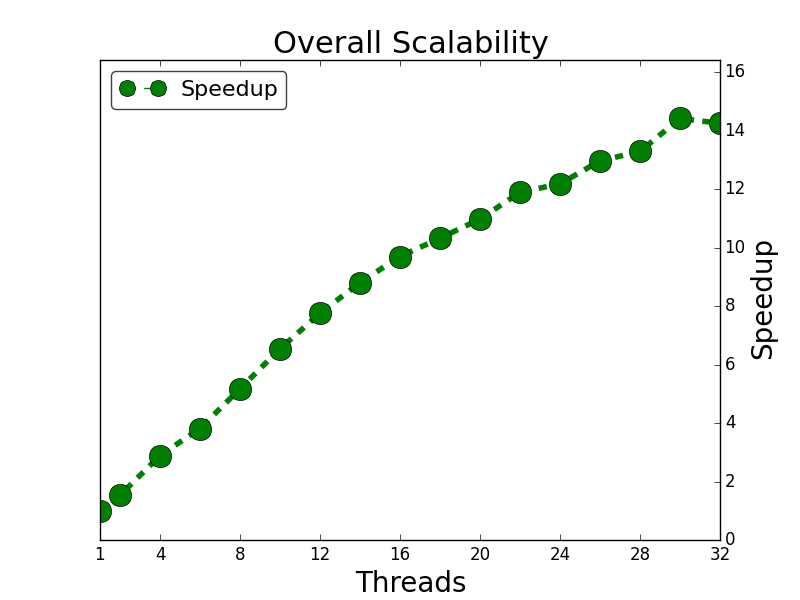
\includegraphics[width=\plotsize\textwidth]{experiments/scalability/overview.png}
        \mycap{Overall scalability for the benchmarks presented in this section.
        The average speedup is the weighted harmonic mean using the single threaded
     run time as the weight of each benchmark.}
        \label{fig:evaluation:overview}
\end{figure}


We now analyze each program separately. For the plots presented next, the $x$
axis represents the number of threads used, the left $y$ axis represents the run
time (in milliseconds) for that particular configuration and uses a logarithmic
scale and the right axis $y$ represents the speedup computed as $T_1/T_i$, where
$T_i$ represents the run time of the program using $i$ threads.  In some plots,
there is also an horizontal black line that represents the run time of the C++
program and is used to understand how many threads are needed in order for an LM
program to run faster than the C++ program. Note that all run times are the
average of three runs.

The scalability results for the Belief Propagation program are presented in
Fig.~\ref{fig:implementation:scale_bp}. This program has the best scalability
with a 60-fold speedup for 32 threads. This is because the default ordering used
for 1 thread is not optimal, while the same ordering works better for multiple
threads. Additionally, the existence of multiple threads increase the amount of
up-to-date information from neighbor nodes, resulting in super-linear speedups.
Note that we also used the same computation ordering in the C++ program, which
is also the one used in the GraphLab framework.

\begin{figure}[]
        \centering
        \begin{subfigure}[b]{\plotsize\textwidth}
                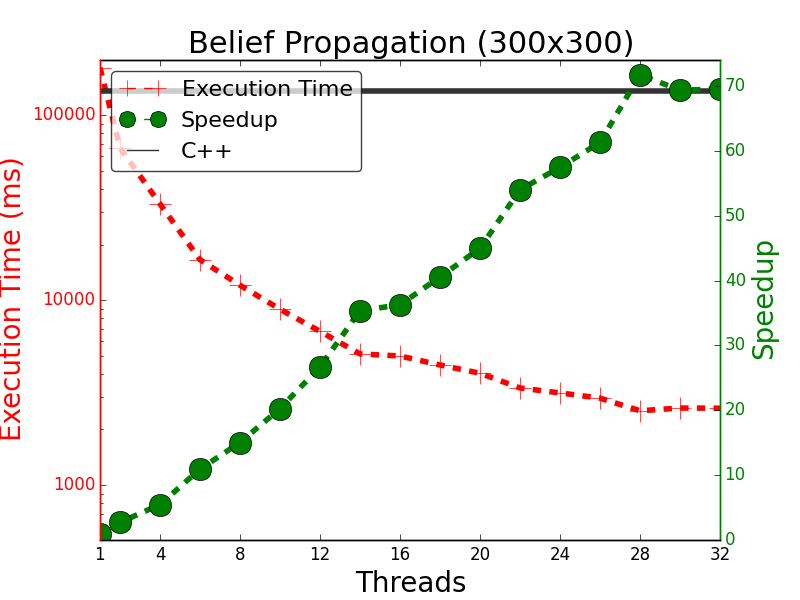
\includegraphics[width=\textwidth]{experiments/scalability/scale-belief-propagation-300.png}
                \label{fig:implementation:scale_bp300}
        \end{subfigure}
        ~
        \begin{subfigure}[b]{\plotsize\textwidth}
                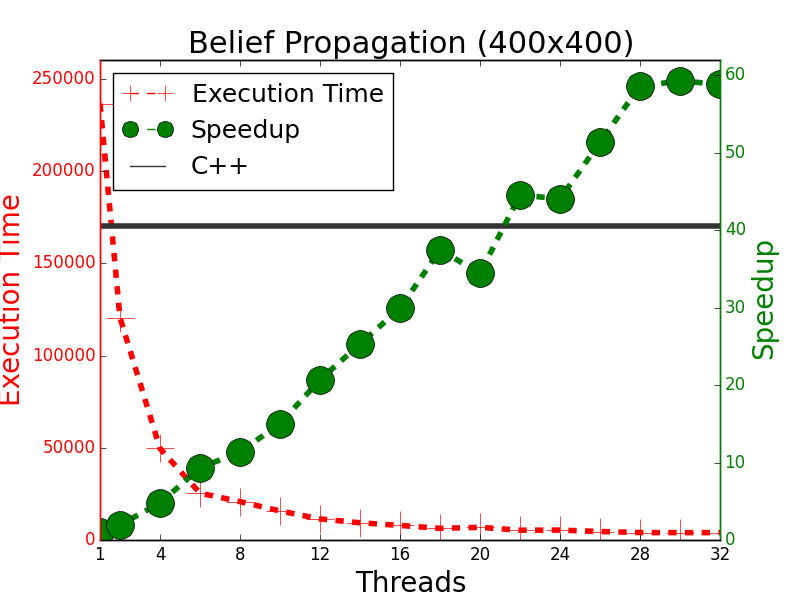
\includegraphics[width=\textwidth]{experiments/scalability/scale-belief-propagation-400.png}
                \label{fig:implementation:scale_bp400}
        \end{subfigure}\\
        \mycap{Scalability results of the Belief Propagation program.}
        \label{fig:implementation:scale_bp}
\end{figure}

The results for the Heat Transfer program are shown in
Fig.~\ref{fig:implementation:scale_ht}. We note that LM requires around 15
threads to reach the run time of the C++ program. This results from the poor
absolute performance of the LM program that was mentioned in the previous section.
Although we use a grid dataset, the work available in the graph is not equally
distributed due to different initial heat values, therefore an almost linear
speedup should not be expected. When comparing the two datasets used, the 80x80
configuration has less scalability than the 120x120 dataset due to its smaller
size. For the 120x120 dataset, LM has a 12-fold speedup for 32 threads, which
makes the LM version run almost twice as fast as the C++ version.

\begin{figure}[]
        \begin{subfigure}[b]{\plotsize\textwidth}
                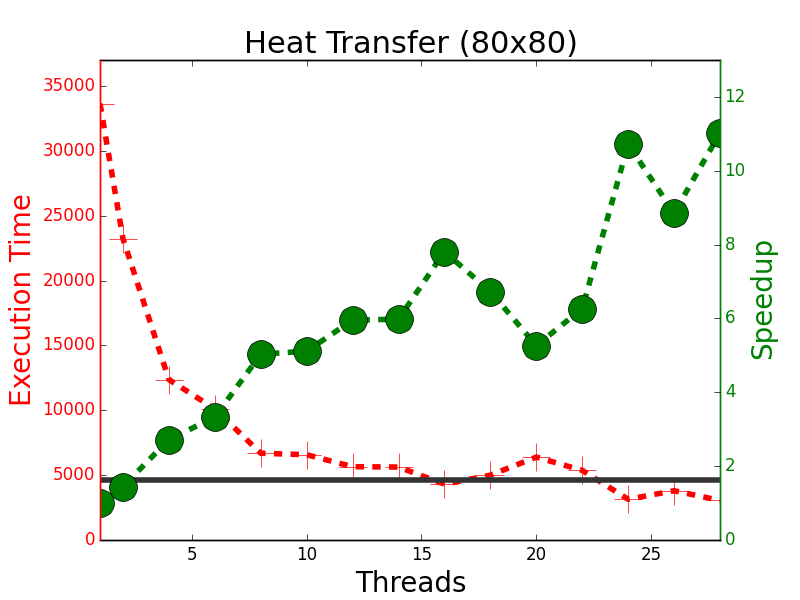
\includegraphics[width=\textwidth]{experiments/scalability/scale-new-heat-transfer-80.png}
                \label{fig:implementation:scale_ht80}
        \end{subfigure}
        ~
        \begin{subfigure}[b]{\plotsize\textwidth}
                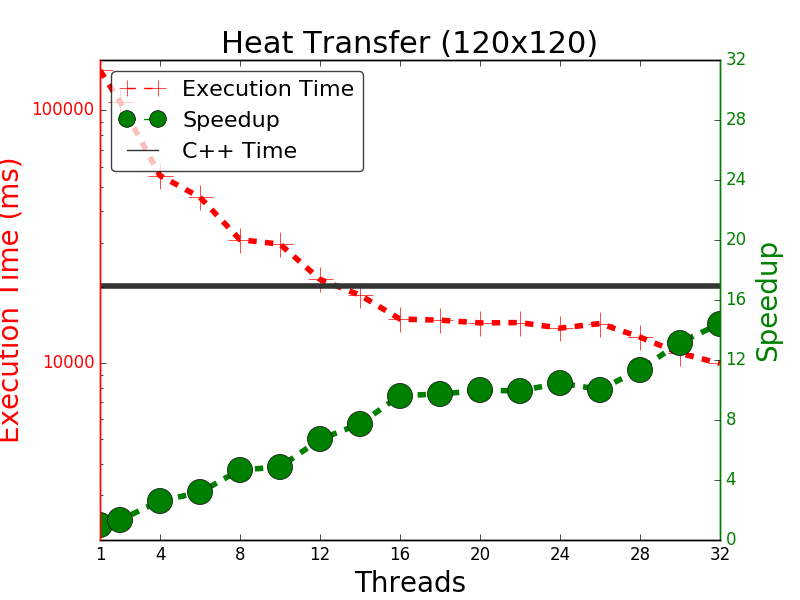
\includegraphics[width=\textwidth]{experiments/scalability/scale-new-heat-transfer-120.png}
                \label{fig:implementation:scale_ht120}
        \end{subfigure}\\
        \mycap{Scalability results for the Heat Transfer program. Because the
           Heat Transfer program performs poorly when compared to the C++ program,
           the LM version needs at least 15 threads to reach the run time of the C++
           program (for the 120x120 dataset).}
        \label{fig:implementation:scale_ht}
\end{figure}

Figure~\ref{fig:implementation:scale_ggc} presents the results for the Greedy
Graph Coloring~(GGC) program. In GGC, we use two datasets: Google
Plus~\cite{snapnets}, a graph representing social circles in Google Plus with
107614 nodes and 13673453 edges, and Twitter, a graph representing Twitter
networks with 81306 nodes and 1768149 edges (note that Twitter was also used
before in the MSSD program). The Twitter and Google Plus datasets have almost
the same number of nodes but Google Plus has ten times more edges, which makes
coloring more time consuming. Since Twitter is a much smaller dataset, its
speedup is much smaller than Google Plus, as expected. However, while the
speedup of Twitter starts to drop after 16 threads, the LM system is still able
to make it faster by adding more threads. For Google Plus, a 20-fold speedup is
achieved for 32 threads, which is a reasonable scalability considering that GGC
is not a program where work is equally distributed.

\begin{figure}[]
        \begin{subfigure}[b]{\plotsize\textwidth}
                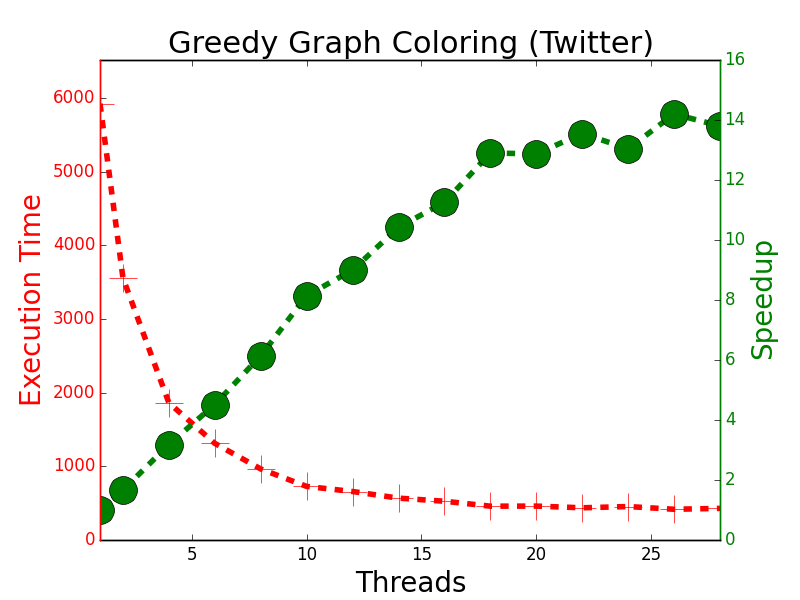
\includegraphics[width=\textwidth]{experiments/scalability/scale-greedy-graph-coloring-twitter.png}
                \label{fig:implementation:scale_ggc_twitter}
        \end{subfigure}
        ~
        \begin{subfigure}[b]{\plotsize\textwidth}
                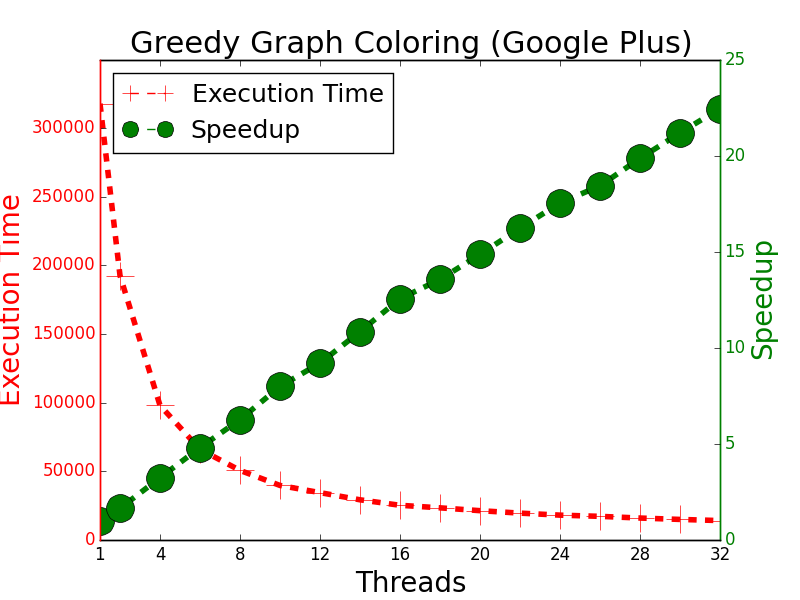
\includegraphics[width=\textwidth]{experiments/scalability/scale-greedy-graph-coloring-gplus.png}
                \label{fig:implementation:scale_ggc_gplus}
        \end{subfigure}\\

        \mycap{Scalability of the Greedy Graph Coloring program.}

        \label{fig:implementation:scale_ggc}
\end{figure}

The results for the N-Queens program are shown in
Fig.~\ref{fig:implementation:scale_queens}. We decided to just use the 13 and 14
configurations since those take longer to run. The 13-Queens configuration has
169 (13x13) nodes while the 14-Queens configuration has 196 (14x14) nodes. The LM program
considers the chess board as a graph and the bottom rows have more work to
perform since the valid queens placements are built from the top to the bottom
row. For a more in-depth explanation of the N-Queens program please see
Section~\ref{section:coord:nqueens}.

Due to the small number of nodes in the N-Queens program and the fact that more
work is performed at the bottom rows, the N-Queens program is hard to
parallelize. Furthermore, the solutions for the puzzle are built by constructing
lists which are shared between threads. This introduces some potential false
sharing because the reference count of each list data structure needs to be
updated when new solutions are constructed. The 14-Queens configuration has good
efficiency using 16 to 20 threads, while the 13-Queens configuration efficiency
starts to drop after 14 threads. One can argue that the best number of threads
is correlated to the size of the board, because the second half of execution is
better balanced and partitioned when the number of threads matches the size of
the board.

\begin{figure}[]
        \centering
        \begin{subfigure}[b]{\plotsize\textwidth}
                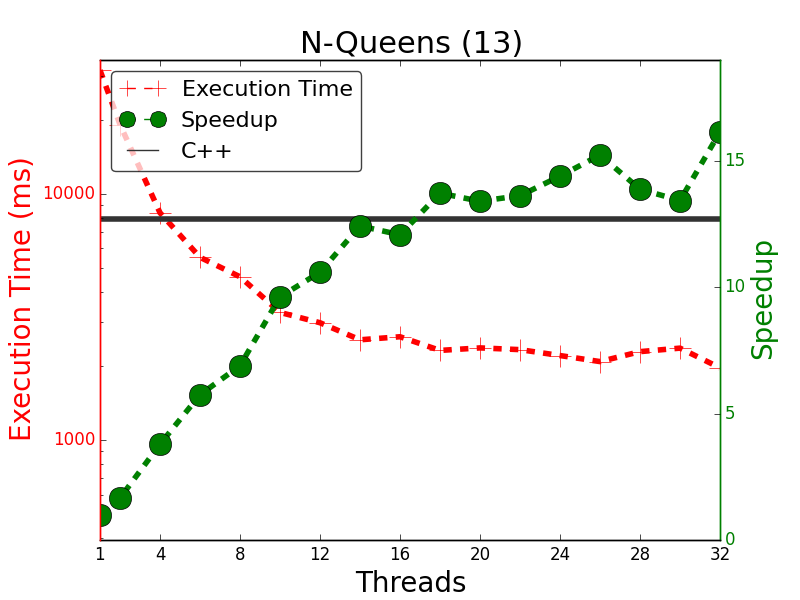
\includegraphics[width=\textwidth]{experiments/scalability/scale-8queens-13.png}
                \label{fig:implementation:scale_queens13}
        \end{subfigure}
        ~
        \begin{subfigure}[b]{\plotsize\textwidth}
                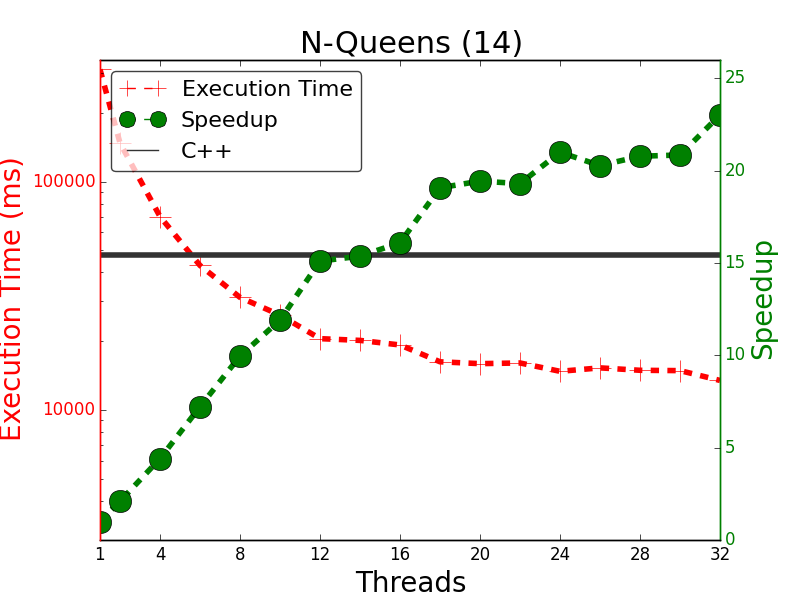
\includegraphics[width=\textwidth]{experiments/scalability/scale-8queens-14.png}
                \label{fig:implementation:scale_queens14}
        \end{subfigure}

        \mycap{Scalability results for the N-Queens program. The 13
        configuration has 73712 solutions, while the 14 configuration has 365596
     solutions. In terms of graph size, the 13 configuration has $13 \times 13$
  nodes while the 14 configuration has $14 \times 14$ nodes.}

        \label{fig:implementation:scale_queens}
\end{figure}

The speedup results for the MiniMax program is shown in
Fig.~\ref{fig:implementation:scale_minmax}.  This is an interesting program
because the graph is constructed during run time. Furthermore, due to the LM
default scheduling order, the tree is explored in a breadth-first fashion,
requiring the program to hold the complete MiniMax tree in memory. The Big
configuration, for instance, uses, on average, 14GB of memory and a total of
30GB of memory before collecting the tree. Since the machine used for the
experiments has only 32GB, the Small configuration scales better due to the
smaller memory requirements. In Section~\ref{section:coord:minimax}, we will
show how this program can be improved by changing the default scheduling order
of LM and improving the memory usage of the program.

\begin{figure}[]
        \begin{subfigure}[b]{\plotsize\textwidth}
                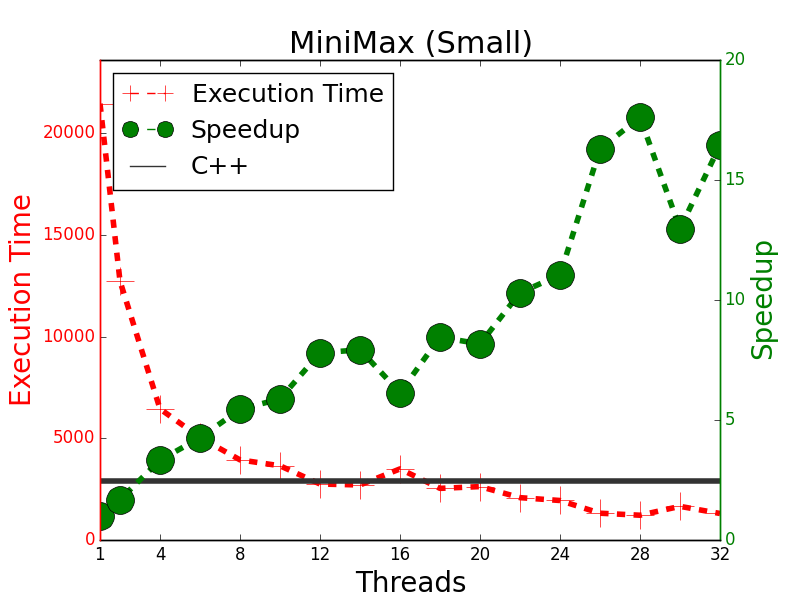
\includegraphics[width=\textwidth]{experiments/scalability/scale-min-max-tictactoe-small.png}
                \label{fig:implementation:scale_minmax_small}
        \end{subfigure}
        ~
        \begin{subfigure}[b]{\plotsize\textwidth}
                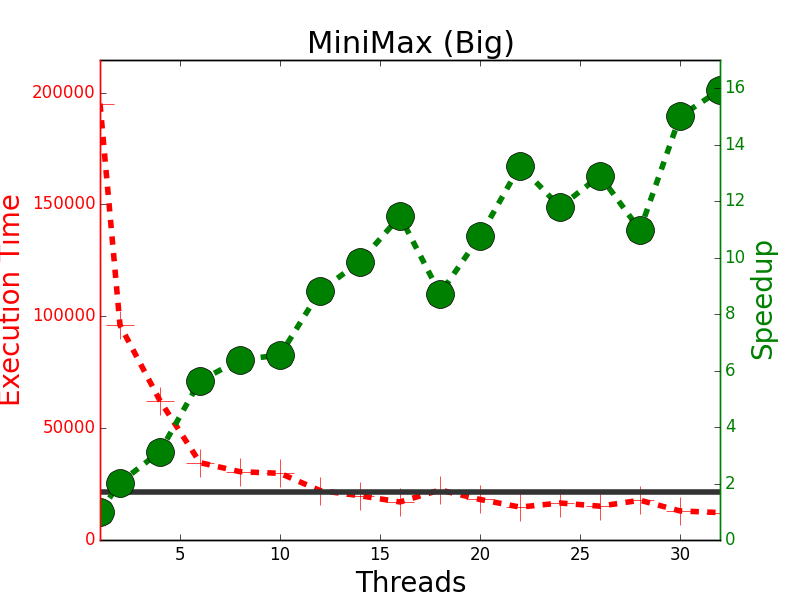
\includegraphics[width=\textwidth]{experiments/scalability/scale-min-max-tictactoe-big.png}
                \label{fig:implementation:scale_minmax_big}
        \end{subfigure}\\

        \mycap{Scalability for the MiniMax program. Although the Big
           configuration has more work available and could in principle scale
           better than Small, the high memory requirements of Big makes it scale
           poorly.}

        \label{fig:implementation:scale_minmax}
\end{figure}

The scalability results for the MSSD program are shown in
Fig.~\ref{fig:implementation:scale_sssp}. The amount of work required to compute
the results of each dataset depends on the size of the graph and the number of
nodes from which the distance must be computed. The first conclusion is that
more work implies more scalability, and the US Power Grid dataset has a 20-fold
speedup for 32 threads, the best from the 6 datasets used. The second conclusion
is that all datasets are able to, at least, reach the execution speed of the
corresponding C++ program. However, some datasets such as EU Email or Orkut, are
notoriously faster than C++ when using more than 5 threads, which is a
impressive result.  We think this is because the number of source nodes is
small. Furthermore, LM as a slight advantage over the C++ program because, in
LM, distances to different nodes are propagated at once, while in the C++
version, the Dijkstra algorithm runs in iterations - one for each node from
which we want to calculate the distance from.

\begin{figure}[]
        \centering
        \begin{subfigure}[b]{\plotsize\textwidth}
                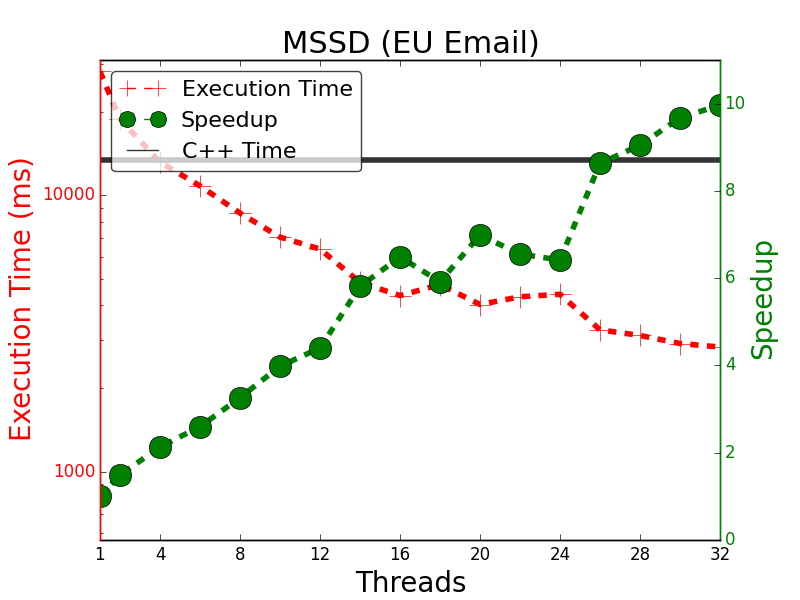
\includegraphics[width=\textwidth]{experiments/scalability/scale-shortest-email.png}
                \label{fig:implementation:scale_sssp_email}
                \mycap{Graph with 265000 nodes and 420000 edges. The shortest
                distance is calculated for 100 nodes.}
        \end{subfigure}
        ~
        \begin{subfigure}[b]{\plotsize\textwidth}
                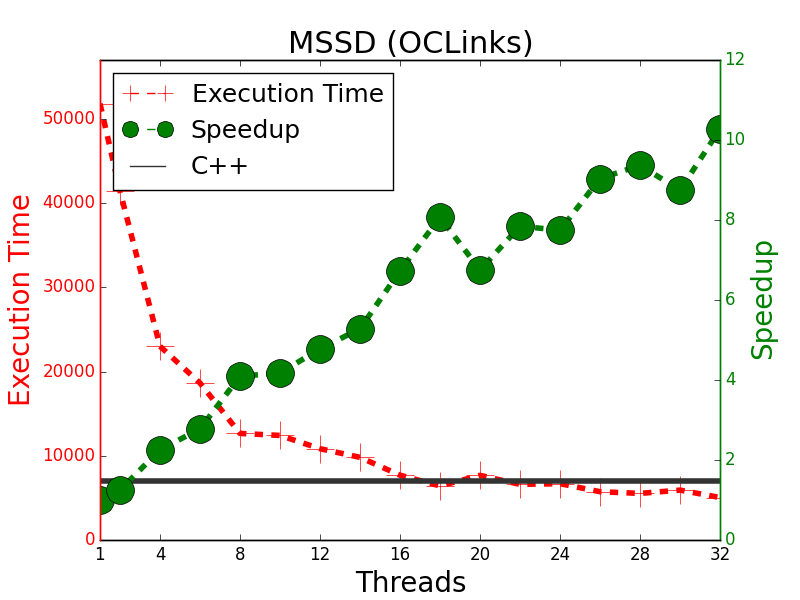
\includegraphics[width=\textwidth]{experiments/scalability/scale-shortest-oclinks.png}
                \label{fig:implementation:scale_sssp_oclinks}
                \mycap{Graph with around 2000 nodes and 20000 edges. The shortest
                   distance is calculated for all nodes.}
        \end{subfigure} \\
        \begin{subfigure}[b]{\plotsize\textwidth}
                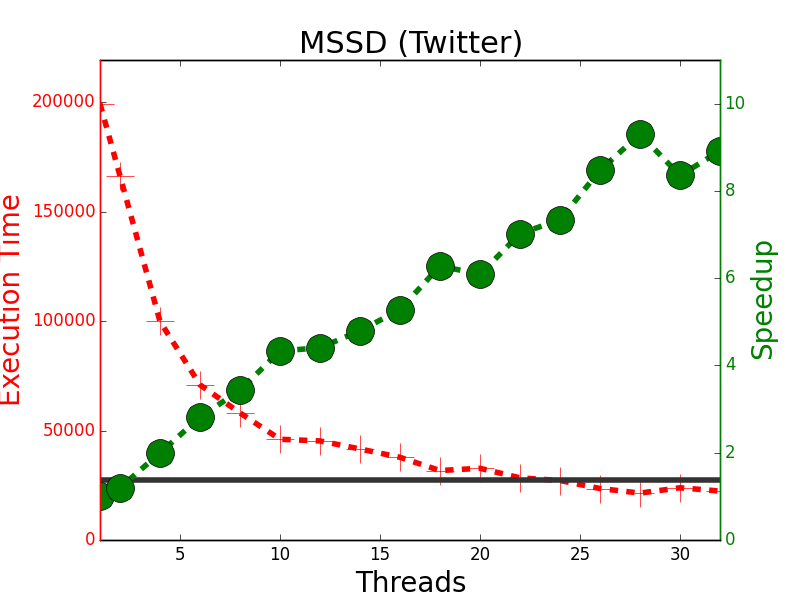
\includegraphics[width=\textwidth]{experiments/scalability/scale-shortest-twitter.png}
                \label{fig:implementation:scale_sssp_twitter}
                \mycap{Graph with 81306 nodes and 1768149 edges. The shortest
                   distance is calculated for 40 nodes.}
        \end{subfigure}
        ~
        \begin{subfigure}[b]{\plotsize\textwidth}
                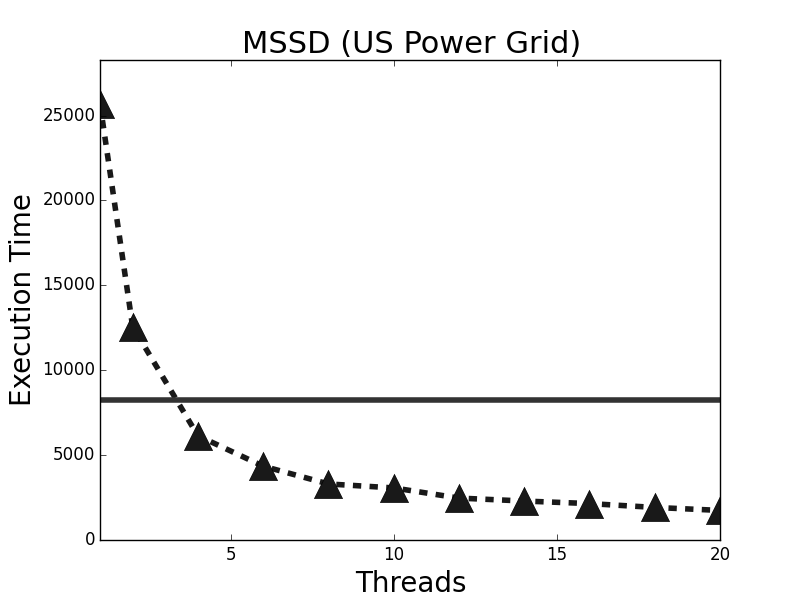
\includegraphics[width=\textwidth]{experiments/scalability/scale-shortest-uspowergrid.png}
                \label{fig:implementation:scale_sssp_uspowergrid}
                \mycap{Graph with around 5000 nodes and 13000 edges. The
                shortest distance is calculated for all nodes.}
        \end{subfigure}\\
        \begin{subfigure}[b]{\plotsize\textwidth}
                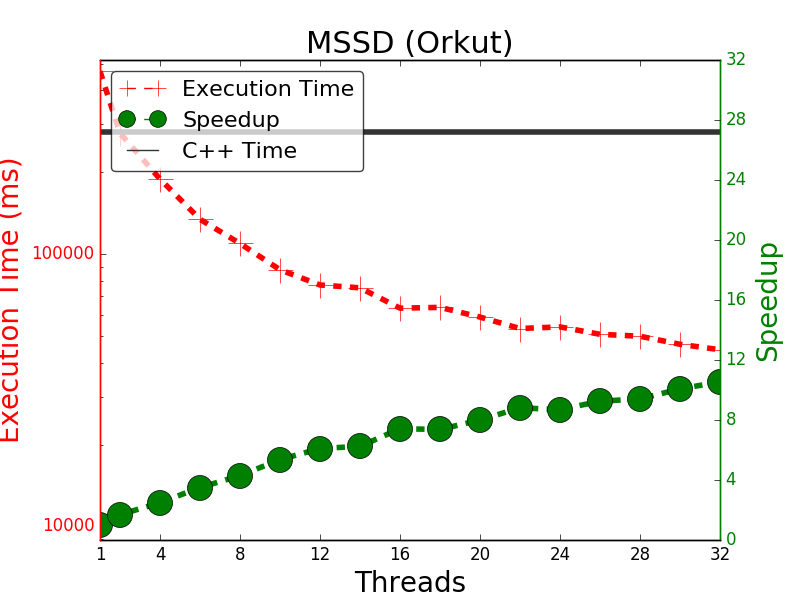
\includegraphics[width=\textwidth]{experiments/scalability/scale-shortest-orkut.png}
                \label{fig:implementation:scale_sssp_orkut}
                \mycap{Graph with 3072441 nodes and 117185083 edges. The shortest
                   distance is calculated for two nodes.}
        \end{subfigure}
        ~
        \begin{subfigure}[b]{\plotsize\textwidth}
                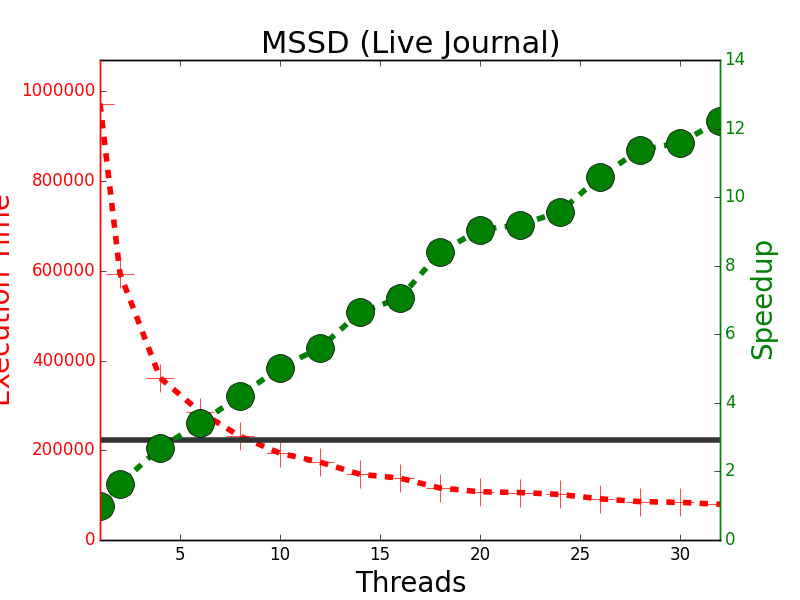
\includegraphics[width=\textwidth]{experiments/scalability/scale-shortest-livejournal.png}
                \label{fig:implementation:scale_sssp_livejournal}
                \mycap{Graph with around 4847571 nodes and 68993773 edges. The
                shortest distance is calculated for two nodes.}
        \end{subfigure}\\

        \mycap{Scalability for the MSSD program. The LM system scales better
        when there is more work to do per node, with the US Power Grid dataset
        showing the most scalability.}

        \label{fig:implementation:scale_sssp}
\end{figure}

The final scalability results are shown for PageRank in
Fig.~\ref{fig:implementation:scale_pagerank}. We used two datasets, Google Plus
and Pokec. Google Plus~\cite{snapnets} has 107614 nodes and 13673453 edges and is based on a Google Plus social network, while Pokec~\cite{snapnets} has
1632803 nodes and 30622564 edges and represents data from a popular social network website in Slovakia.
Even though Pokec is the larger graph, Google
Plus has a denser graph, where the average number of edges per node is 127
compared to the average of 18 for Pokec. This may explain why Google Plus is
more scalable with a 14-fold speedup for 32 threads.

\begin{figure}[]
        \begin{subfigure}[b]{\plotsize\textwidth}
                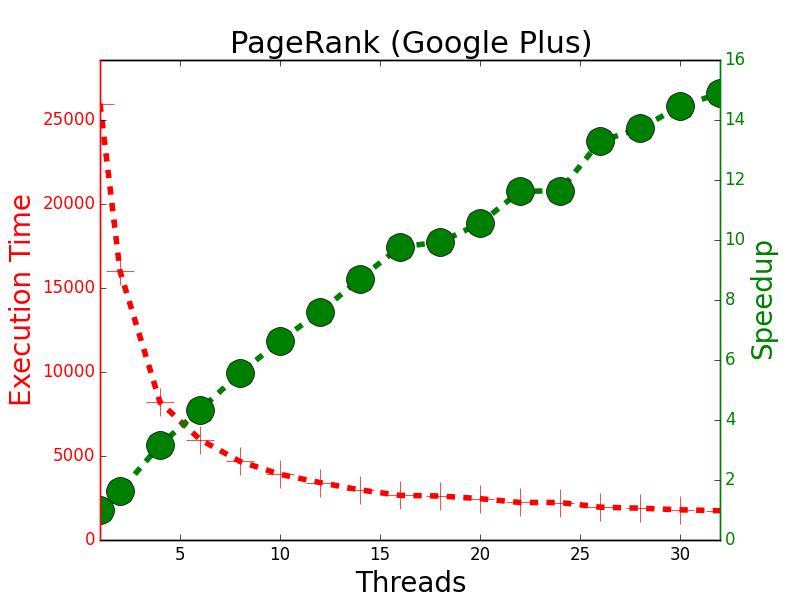
\includegraphics[width=\textwidth]{experiments/scalability/scale-pagerank-gplus.png}
                \label{fig:implementation:scale_pagerank_gplus}
                \mycap{The Google Plus graph has a high average of edges per
                node of 127.}
        \end{subfigure}
        ~
        \begin{subfigure}[b]{\plotsize\textwidth}
                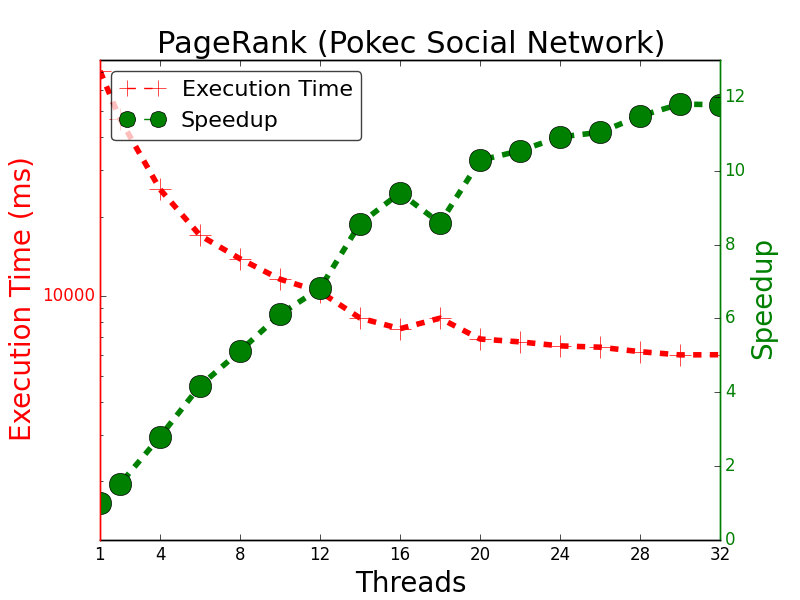
\includegraphics[width=\textwidth]{experiments/scalability/scale-pagerank-pokec.png}
                \label{fig:implementation:scale_pagerank_pokec}
                \mycap{The Pokec graph has a lower average of edges per node
                of 18.}
        \end{subfigure}\\
        \mycap{Scalability results for the asynchronous PageRank program. The
           superior scalability of the Google Plus dataset may be explained by
        its higher density of edges.}
        \label{fig:implementation:scale_pagerank}
\end{figure}


\clearpage

\subsection{Threaded allocator versus \code{malloc}}

In order to understand the role which our threaded allocator plays in the
performance of programs, we evaluate and compare it against the performance of
the LM system by using the \code{malloc} function provided by the operating
system.

Figure~\ref{fig:implementation:malloc_results} presents several programs
comparing \code{malloc} with the threaded allocator. The programs Belief
Propagation, MiniMax, and N-Queens have poor scalability when using the
\code{malloc} operator due to high thread contention when calling \code{malloc}
since those programs need to allocate many small objects. The PageRank programs
shows good scalability with \code{malloc} but it is only because the
configuration with 1 thread runs slowly when compared to the other
configurations. For all the remaining programs, there is less overall
performance and scalability when compared to the threaded allocator.

As these results show, the performance of the memory allocator is crucial for
good performance and scalability. Linear logic programs spend a significant
amount of time asserting and retracting linear facts which require that memory
allocation must be done efficiently and without starving other threads. Reuse of
deallocated linear facts also makes more likely that threads will hit hot cache
lines and thus improve speed significantly.

\newcommand{\smallplotsize}[0]{0.3}

\begin{figure}[h]
        \begin{subfigure}[b]{\smallplotsize\textwidth}
                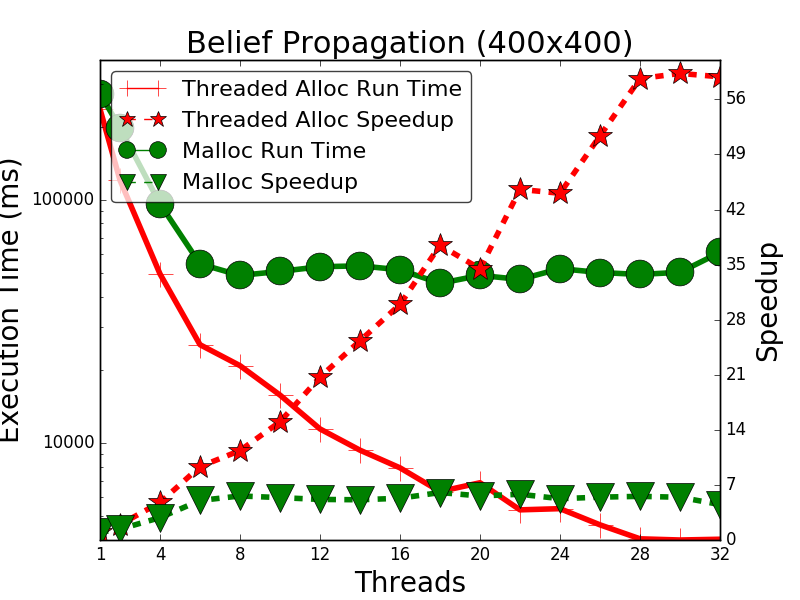
\includegraphics[width=\textwidth]{experiments/scalability/malloc-allocator-belief-propagation-400.png}
                \label{fig:implementation:malloc_bp}
        \end{subfigure}
        ~
        \begin{subfigure}[b]{\smallplotsize\textwidth}
                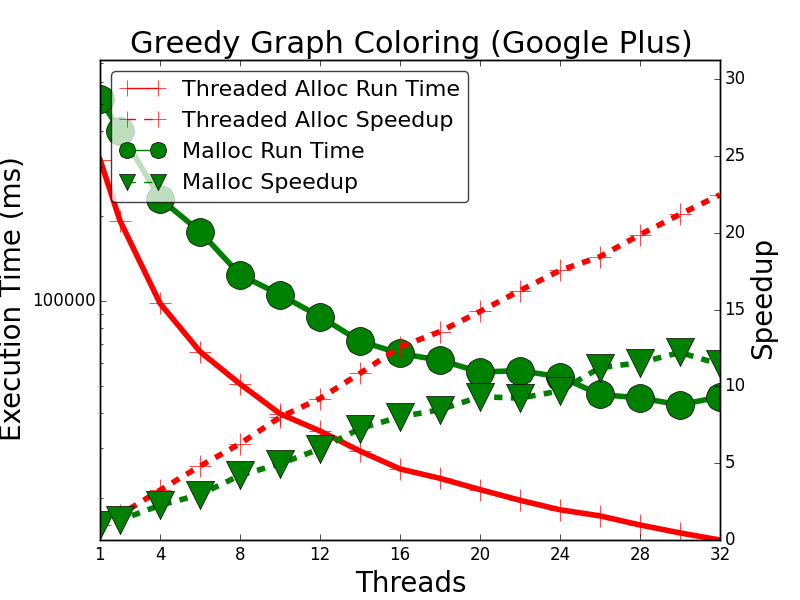
\includegraphics[width=\textwidth]{experiments/scalability/malloc-allocator-greedy-graph-coloring-gplus.png}
                \label{fig:implementation:malloc_ggc}
        \end{subfigure}
        ~
        \begin{subfigure}[b]{\smallplotsize\textwidth}
                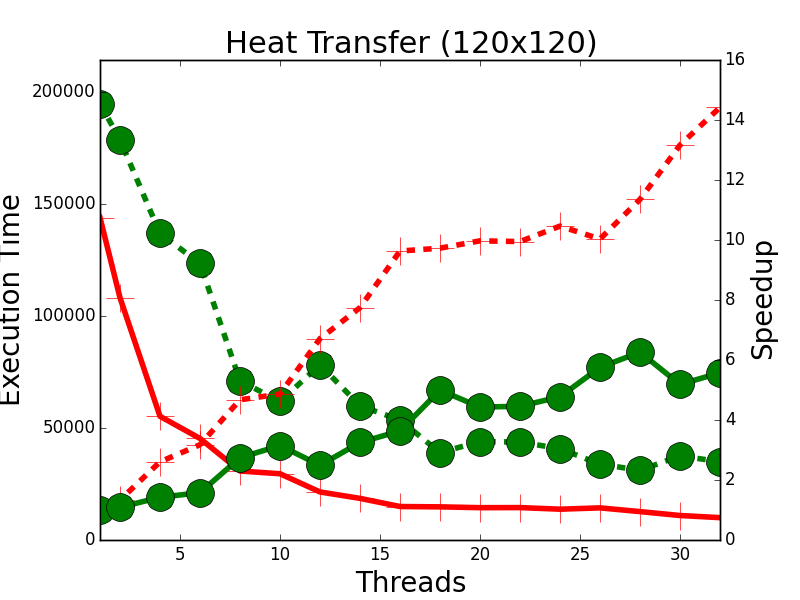
\includegraphics[width=\textwidth]{experiments/scalability/malloc-allocator-new-heat-transfer-120.png}
                \label{fig:implementation:malloc_ht}
        \end{subfigure}
        ~
        \begin{subfigure}[b]{\smallplotsize\textwidth}
                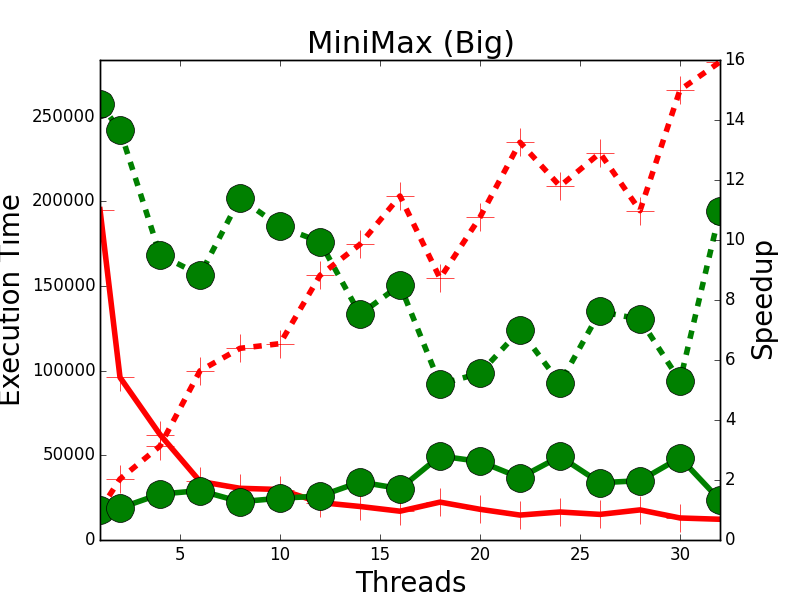
\includegraphics[width=\textwidth]{experiments/scalability/malloc-allocator-min-max-tictactoe-big.png}
                \label{fig:implementation:malloc_minimax}
        \end{subfigure}
        ~
        \begin{subfigure}[b]{\smallplotsize\textwidth}
                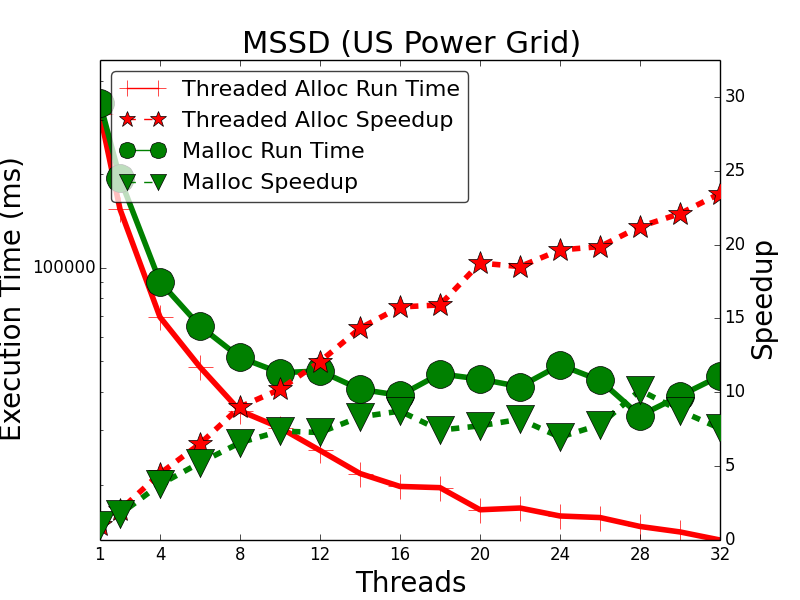
\includegraphics[width=\textwidth]{experiments/scalability/malloc-allocator-shortest-uspowergrid.png}
                \label{fig:implementation:malloc_sssp}
        \end{subfigure}
        ~
        \begin{subfigure}[b]{\smallplotsize\textwidth}
                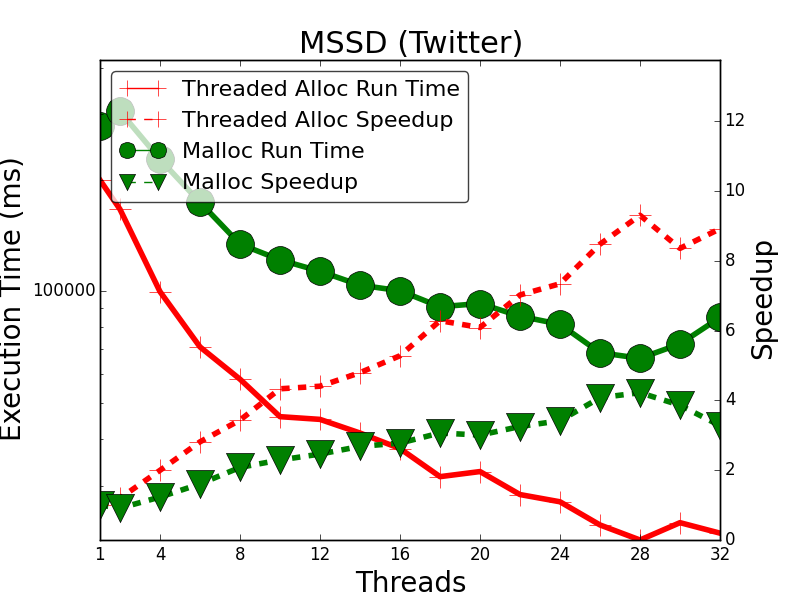
\includegraphics[width=\textwidth]{experiments/scalability/malloc-allocator-shortest-twitter.png}
                \label{fig:implementation:malloc_sssp}
        \end{subfigure}\\
        \begin{subfigure}[b]{\smallplotsize\textwidth}
                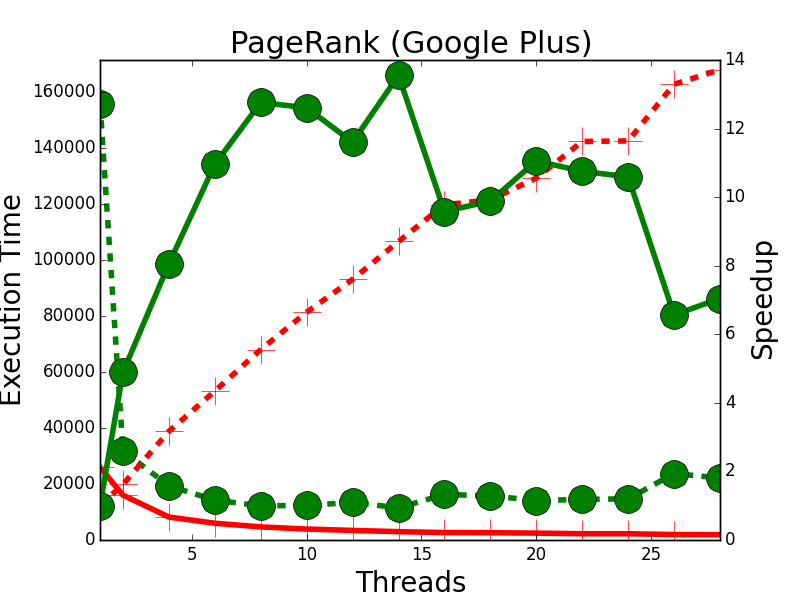
\includegraphics[width=\textwidth]{experiments/scalability/malloc-allocator-pagerank-gplus.png}
                \label{fig:implementation:malloc_pagerank}
        \end{subfigure}
        ~
        \begin{subfigure}[b]{\smallplotsize\textwidth}
                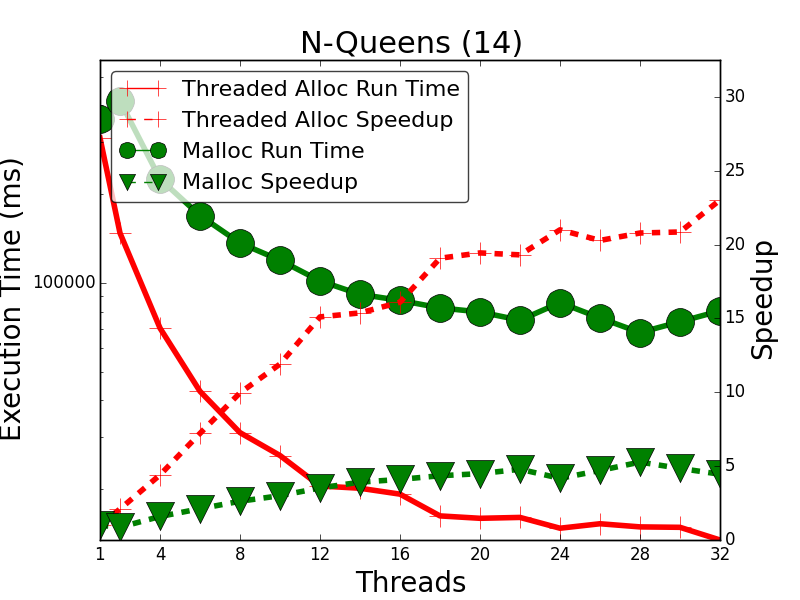
\includegraphics[width=\textwidth]{experiments/scalability/malloc-allocator-8queens-14.png}
                \label{fig:implementation:malloc_queens}
        \end{subfigure} \\

        \mycap{Comparing the threaded allocator described in
           Section~\ref{section:implementation:allocation} against the
           \texttt{malloc} allocator provided by the C library. The threaded
           allocator is represented by plus markers, while \texttt{malloc} is
        represented by circular markers. Note that the two speedup lines (right
     axis) use dashed lines, while the two lines representing the run time (left
  axis) are contiguous.}

        \label{fig:implementation:malloc_results}
\end{figure}


\subsection{Threaded allocator versus node-local allocator}\label{section:implementation:alternative_allocator}
While our default threaded allocator performs and scales well, we also explored
some alternative designs. In this section, we explore a design where we move the
allocation decisions from the thread to the node itself, in order to store the
facts of the same node close together and thus increase locality. However, this
design requires locking since multiple threads may allocate facts from the same
node. Our expectation is that such costs will be offset by the increased
locality and reduced cache misses when deriving rules.

The fact allocator allocates pages of memory from the threaded allocator which
are then used to allocate facts for that particular node. When a thread needs to
allocate or deallocate a fact, it acquires the allocator lock of the target
node's allocator and performs the allocation operation. There is a doubly-linked
list of memory pages and each page contains facts of different sizes
(predicates).

\begin{figure}[ht]
   \begin{center}
      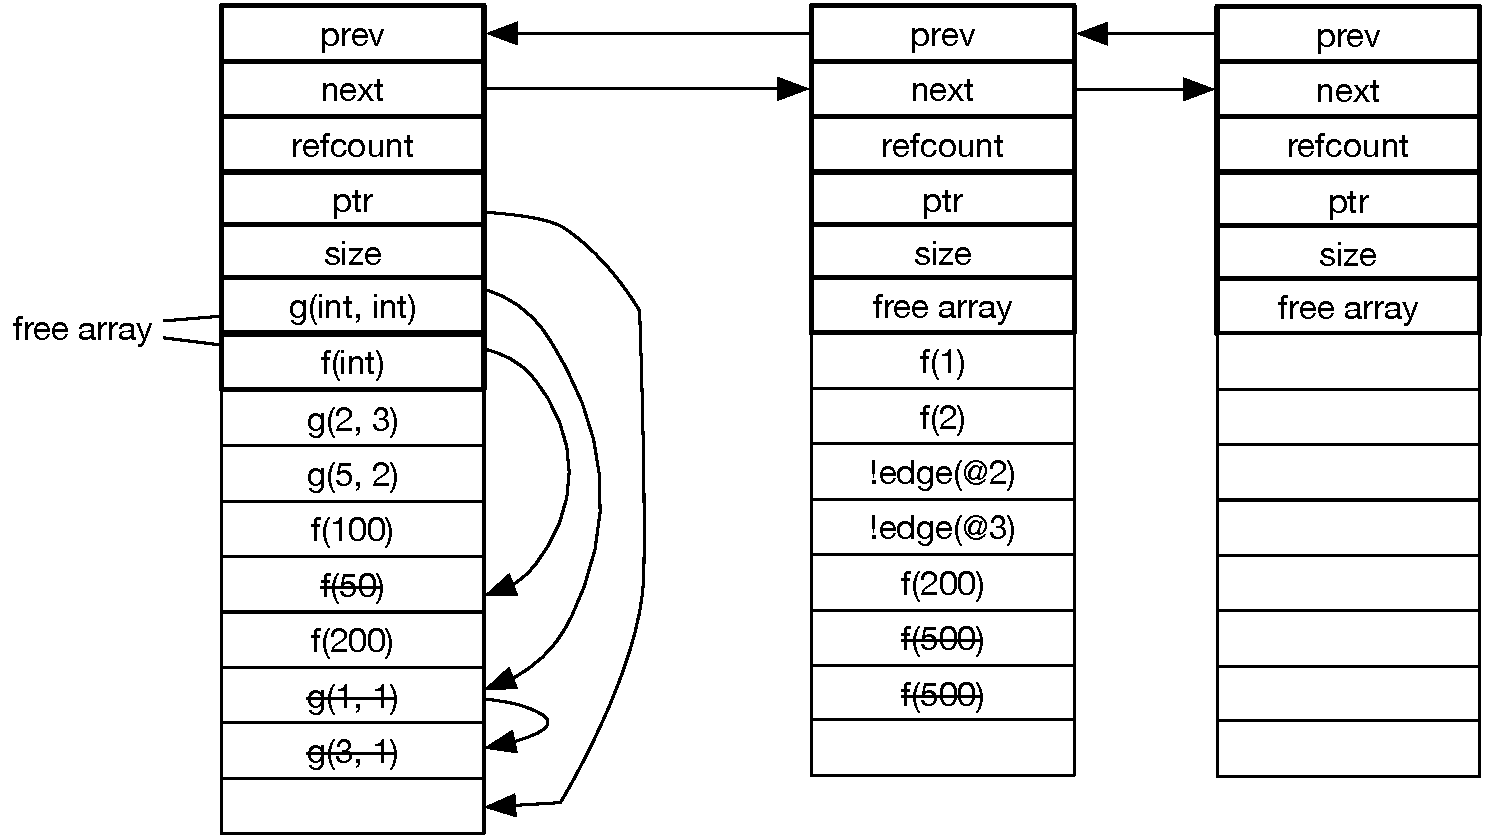
\includegraphics[width=0.7\linewidth]{figures/implementation/fact_allocator.pdf}
   \end{center}

   \mycap{Fact allocator: each node has a pool of memory pages for allocating
      logical facts. Each page contains: (i) several linked lists of free facts
      of the same size (\code{free\_array}); (ii) a reference count of used
      facts (\code{refcount}); (iii) a \code{ptr} pointer that points to
      unallocated space in the page. In this figure, predicates \code{f} and
      \code{g} have several deallocated facts that are ready to be used when a
   new fact needs to be acquired.}

   \label{fig:implementation:fact_allocator}
\end{figure}

Figure~\ref{fig:implementation:fact_allocator} presents an example state of a
fact allocator. The node has 3 memory pages, all connected using the \code{next}
and \code{prev} pointers. Each page also has a reference count (\code{refcount})
of the objects allocated in the page. If the reference count ever drops to zero,
then the memory page is deallocated. Deallocated facts are kept on an ordered
array for different sizes using the mechanism we implemented for the threaded
allocator. We have decided to reference count objects in the fact allocator
because it is more difficult to share objects between nodes and maintaining a
reference count helps reduce memory usage.

Figure~\ref{fig:implementation:node_results} presents the comparison between the
threaded and fact allocator for the most relevant datasets (the performance was
similar for the other datasets).

\begin{figure}[h]
        \begin{subfigure}[b]{\smallplotsize\textwidth}
                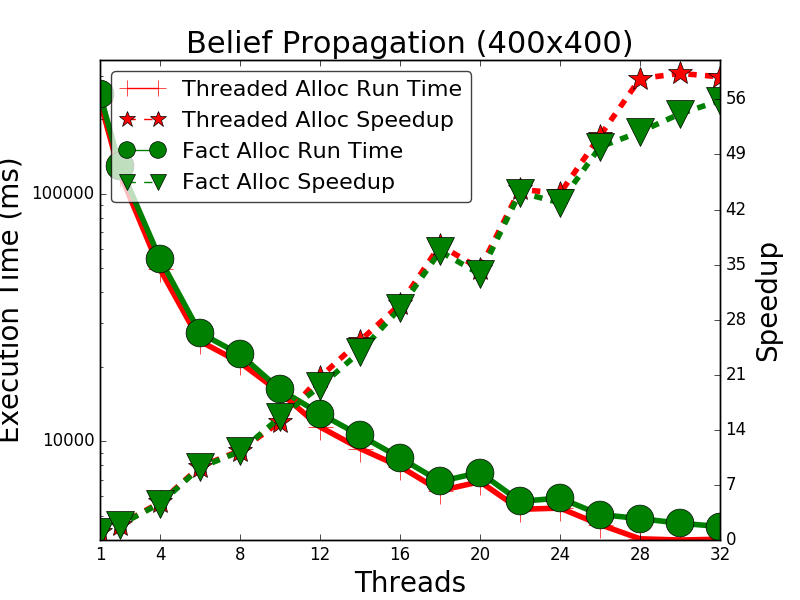
\includegraphics[width=\textwidth]{experiments/scalability/node-allocator-belief-propagation-400.png}
                \label{fig:implementation:node_bp}
        \end{subfigure}
        ~
        \begin{subfigure}[b]{\smallplotsize\textwidth}
                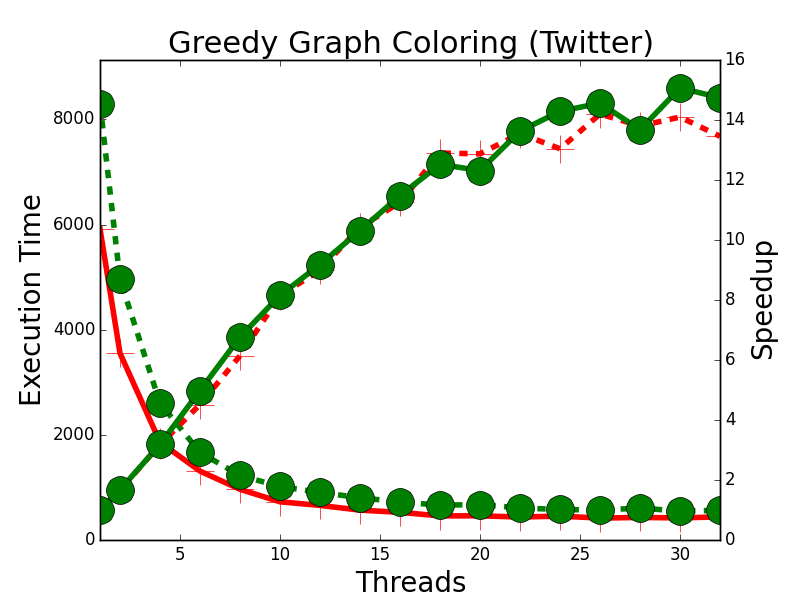
\includegraphics[width=\textwidth]{experiments/scalability/node-allocator-greedy-graph-coloring-twitter.png}
                \label{fig:implementation:node_ggc}
        \end{subfigure}
        ~
        \begin{subfigure}[b]{\smallplotsize\textwidth}
                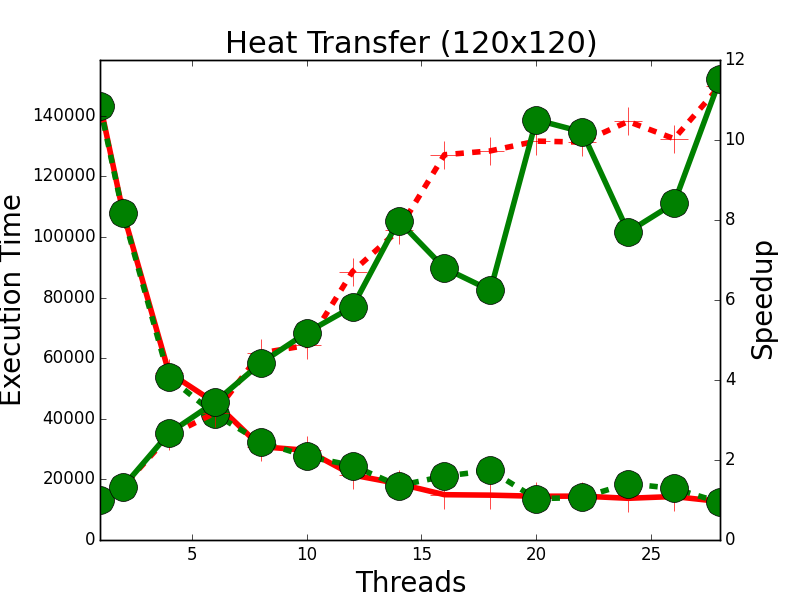
\includegraphics[width=\textwidth]{experiments/scalability/node-allocator-new-heat-transfer-120.png}
                \label{fig:implementation:node_ht}
        \end{subfigure}
        ~
        \begin{subfigure}[b]{\smallplotsize\textwidth}
                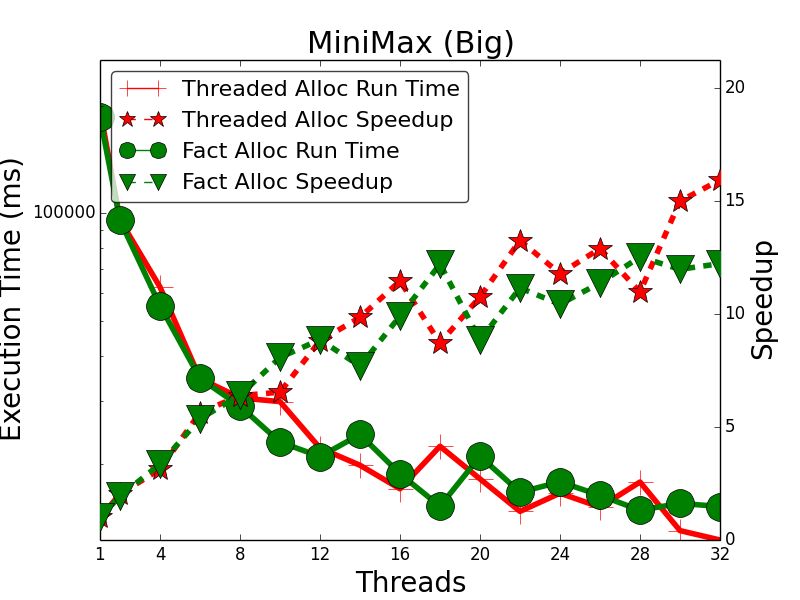
\includegraphics[width=\textwidth]{experiments/scalability/node-allocator-min-max-tictactoe-big.png}
                \label{fig:implementation:node_minimax}
        \end{subfigure}
        ~
        \begin{subfigure}[b]{\smallplotsize\textwidth}
                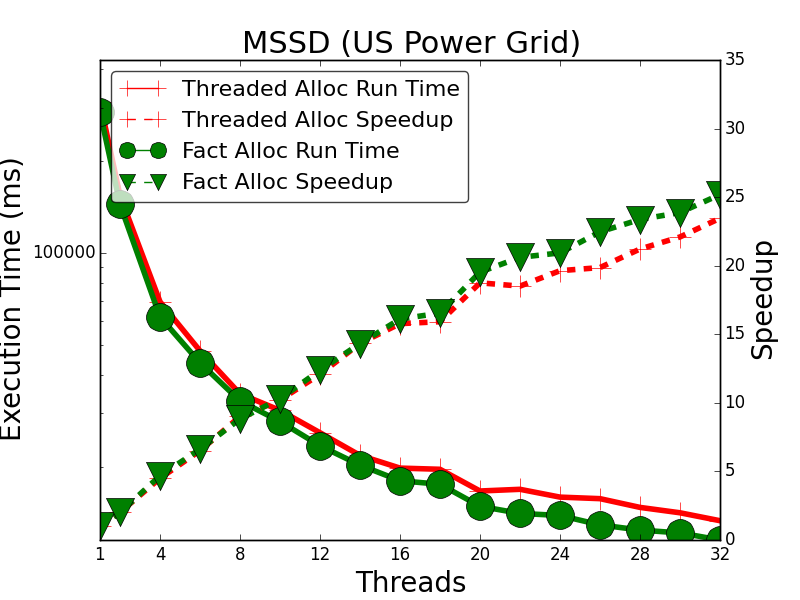
\includegraphics[width=\textwidth]{experiments/scalability/node-allocator-shortest-uspowergrid.png}
                \label{fig:implementation:node_sssp}
        \end{subfigure}
        ~
        \begin{subfigure}[b]{\smallplotsize\textwidth}
                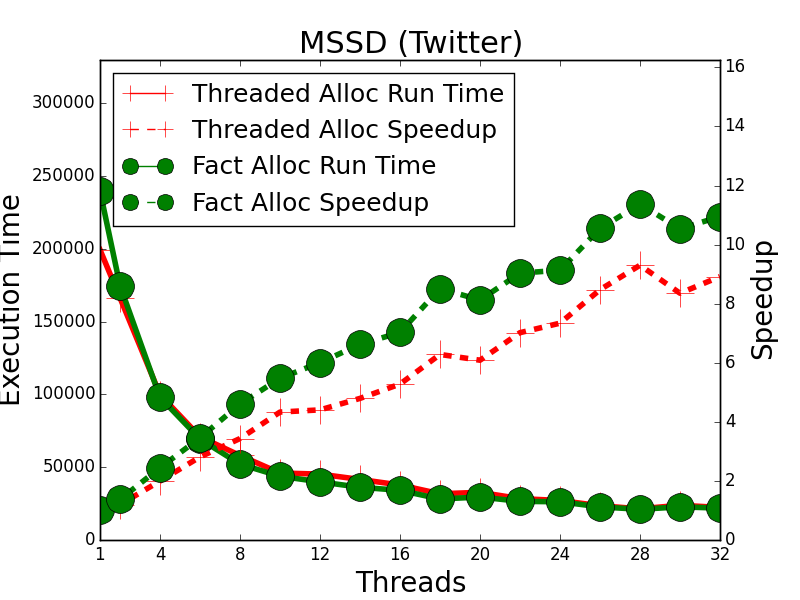
\includegraphics[width=\textwidth]{experiments/scalability/node-allocator-shortest-twitter.png}
                \label{fig:implementation:node_sssp2}
        \end{subfigure}\\
        \begin{subfigure}[b]{\smallplotsize\textwidth}
                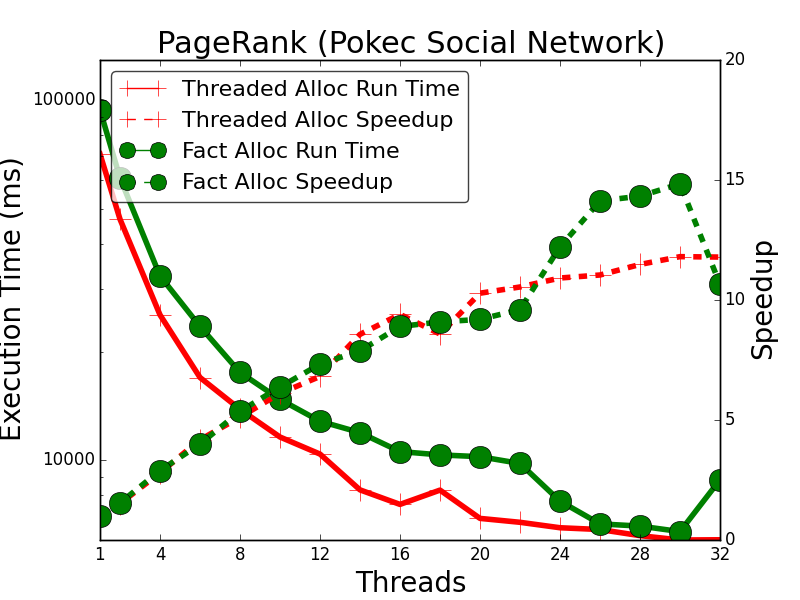
\includegraphics[width=\textwidth]{experiments/scalability/node-allocator-pagerank-pokec.png}
                \label{fig:implementation:node_pagerank}
        \end{subfigure}
        ~
        \begin{subfigure}[b]{\smallplotsize\textwidth}
                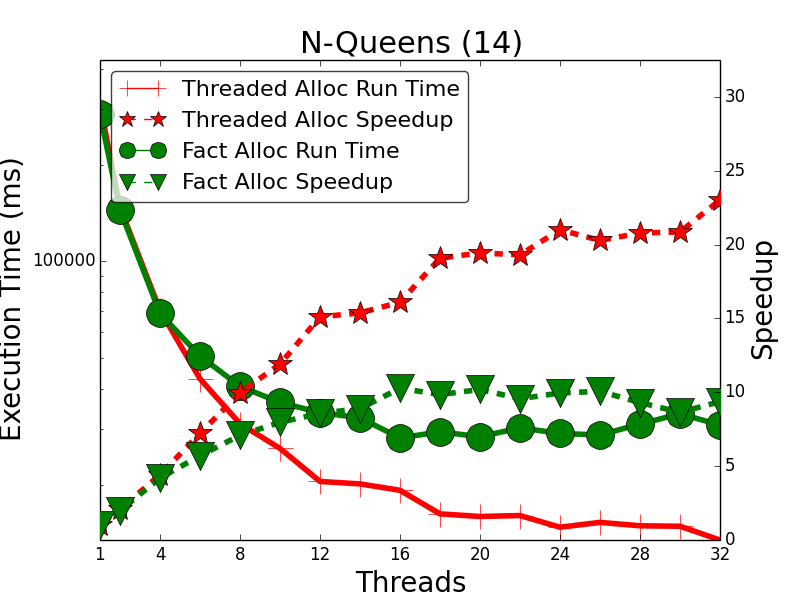
\includegraphics[width=\textwidth]{experiments/scalability/node-allocator-8queens-14.png}
                \label{fig:implementation:node_queens}
        \end{subfigure} \\
        \mycap{Comparing the threaded allocator described in
        Section~\ref{section:implementation:allocation} against the fact
     allocator.}

        \label{fig:implementation:node_results}
\end{figure}

The first major observation from the comparison is that the threaded allocator
has better sequential performance than the fact allocator for most programs.
This is probably the result of better locality for the threaded allocator
because it does not need to create pages for each node and instead uses the
thread pages to maintain all facts, reducing cache line misses. Overall, the
performance of the threaded allocator is better or similar than the fact
allocator, for both single and multithreaded threaded execution (see GGC for a
clear example).

The second observation is in the N-Queens program, where the threaded allocator
beats the fact allocator by a high margin in terms of scalability and
performance. Note that the N-Queens program allocates many of lists and those
lists are not allocated on a per node basis but on a thread basis, therefore the
extra work required to maintain each fact allocator is not offset by the
increased locality because the threads need to traverse lists to find valid
board states.

To make our comparison more interesting, we also deactivated the reference
counting mechanisms of the fact allocator and compared it against the threaded
allocator. The goal is to understand how reference counting affects the
performance of the alternative allocator. The complete comparison are shown in
Fig.~\ref{fig:implementation:no_refs_results}. In a nutshell, it performs almost
the same as the full featured fact allocator, except for programs which require
more memory such as MiniMax and Heat Transfer. In the case of MiniMax, we were
unable to completely execute the Big dataset since the VM required more memory
than the available memory, resulting in long execution times. This is the result
of not collecting unused memory pages, which results in high memory usage.


\begin{figure}[h]
        \begin{subfigure}[b]{\smallplotsize\textwidth}
                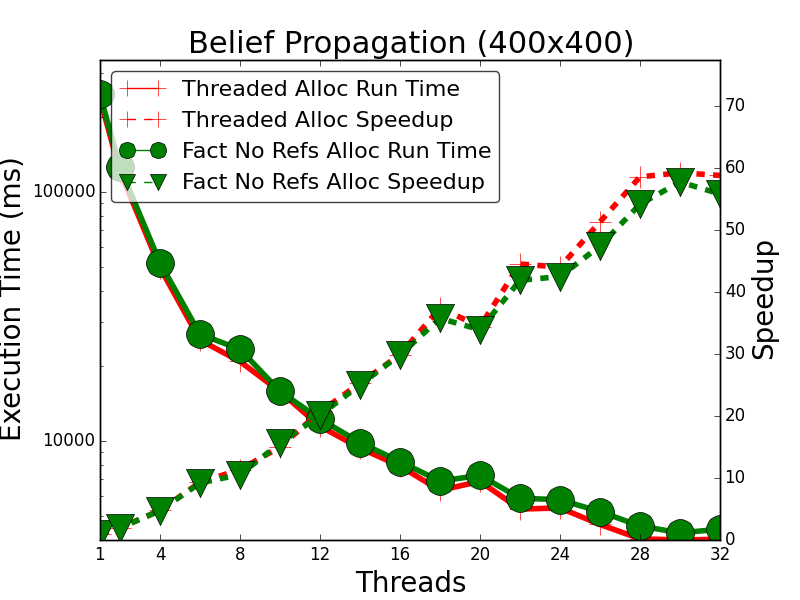
\includegraphics[width=\textwidth]{experiments/scalability/no-refs-allocator-belief-propagation-400.png}
                \label{fig:implementation:no_refs_bp}
        \end{subfigure}
        ~
        \begin{subfigure}[b]{\smallplotsize\textwidth}
                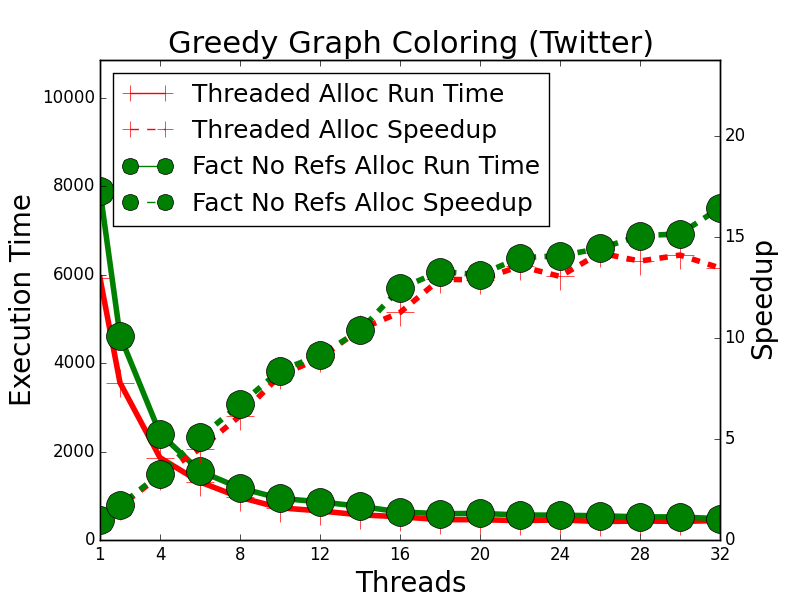
\includegraphics[width=\textwidth]{experiments/scalability/no-refs-allocator-greedy-graph-coloring-twitter.png}
                \label{fig:implementation:no_refs_ggc}
        \end{subfigure}
        ~
        \begin{subfigure}[b]{\smallplotsize\textwidth}
                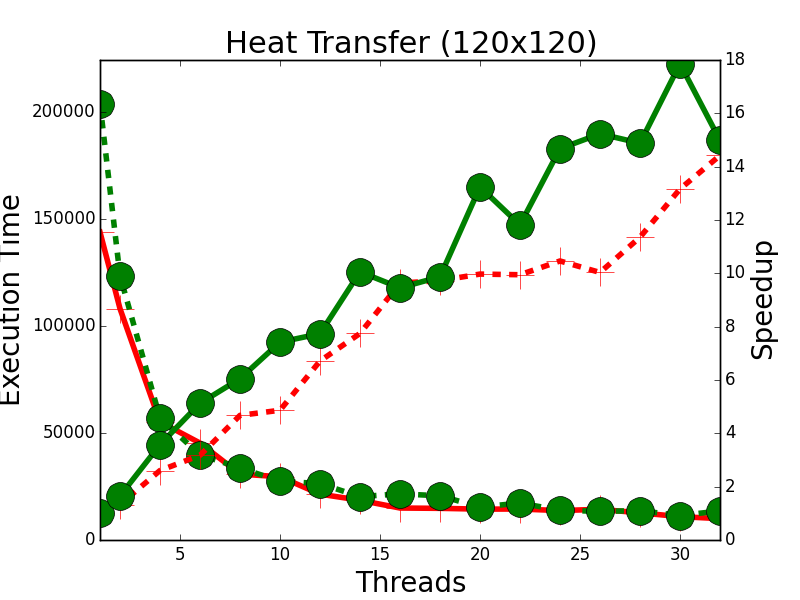
\includegraphics[width=\textwidth]{experiments/scalability/no-refs-allocator-new-heat-transfer-120.png}
                \label{fig:implementation:no_refs_ht}
        \end{subfigure}
        ~
        \begin{subfigure}[b]{\smallplotsize\textwidth}
                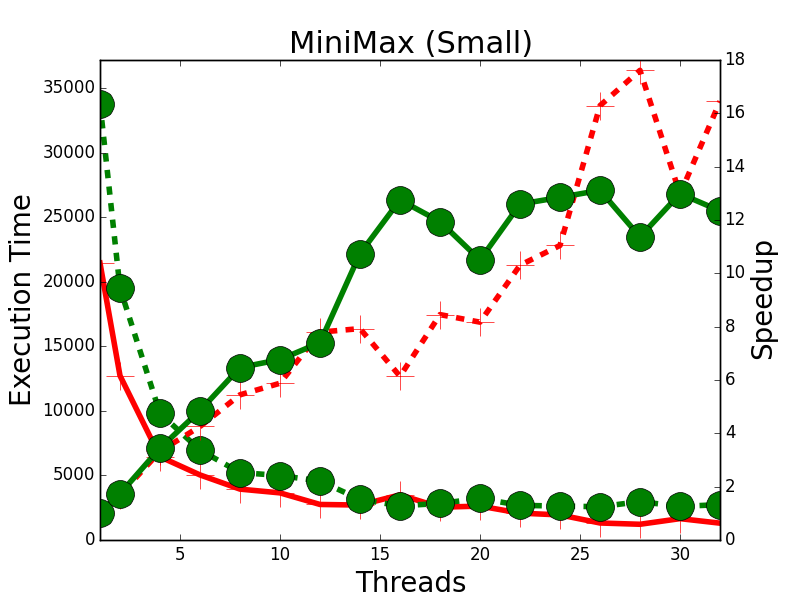
\includegraphics[width=\textwidth]{experiments/scalability/no-refs-allocator-min-max-tictactoe-small.png}
                \label{fig:implementation:no_refs_minimax}
        \end{subfigure}
        ~
        \begin{subfigure}[b]{\smallplotsize\textwidth}
                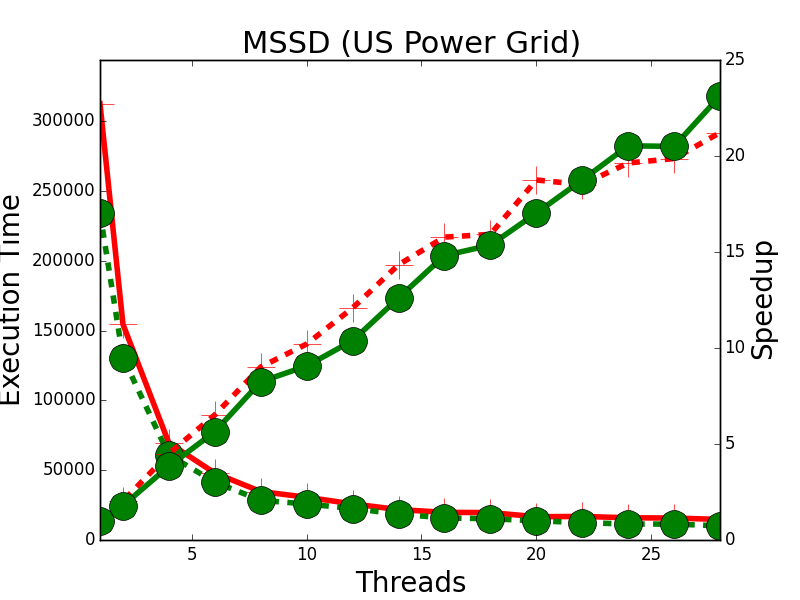
\includegraphics[width=\textwidth]{experiments/scalability/no-refs-allocator-shortest-uspowergrid.png}
                \label{fig:implementation:no_refs_sssp}
        \end{subfigure}
        ~
        \begin{subfigure}[b]{\smallplotsize\textwidth}
                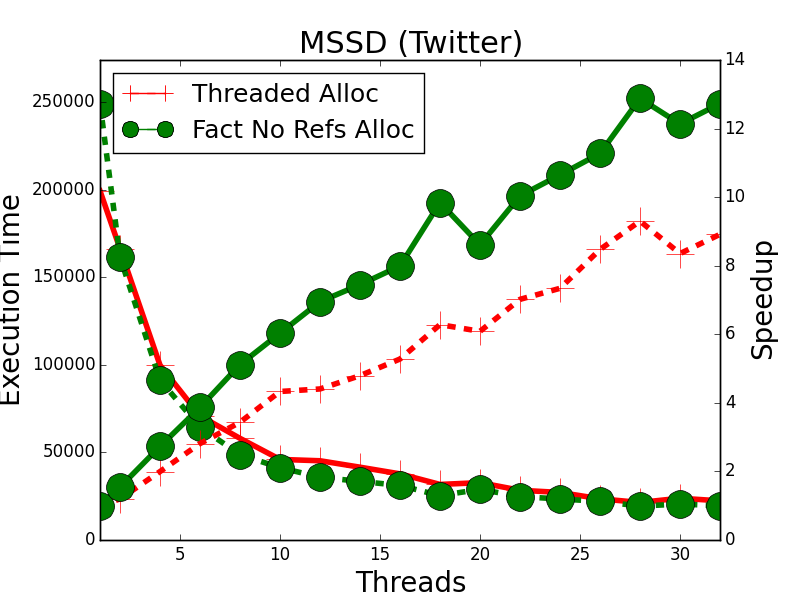
\includegraphics[width=\textwidth]{experiments/scalability/no-refs-allocator-shortest-twitter.png}
                \label{fig:implementation:no_refs_sssp2}
        \end{subfigure}\\
        \begin{subfigure}[b]{\smallplotsize\textwidth}
                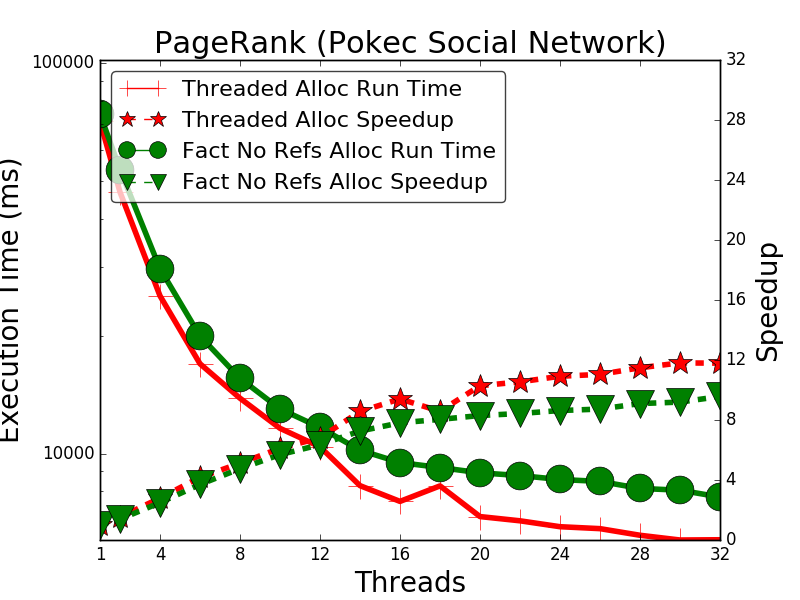
\includegraphics[width=\textwidth]{experiments/scalability/no-refs-allocator-pagerank-pokec.png}
                \label{fig:implementation:no_refs_pagerank}
        \end{subfigure}
        ~
        \begin{subfigure}[b]{\smallplotsize\textwidth}
                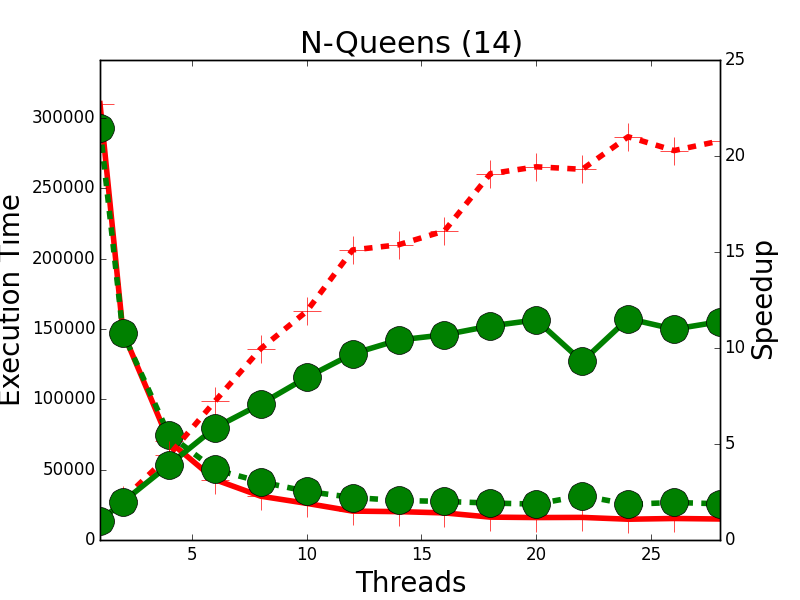
\includegraphics[width=\textwidth]{experiments/scalability/no-refs-allocator-8queens-14.png}
                \label{fig:implementation:no_refs_queens}
        \end{subfigure} \\

        \mycap{Comparing the threaded allocator described in
           Section~\ref{section:implementation:allocation} against the fact
        allocator without reference counting.}

        \label{fig:implementation:no_refs_results}
\end{figure}


Overall, the performance of both allocators is similar, therefore we have
decided to use the threaded allocator by default since it is simpler and offers
good performance across the board. Furthermore, the threaded allocator requires
less allocated memory because it enables more sharing between nodes.


